% Kerswell et al. Coupling G3 submission June 2020
\documentclass[draft]{assets/agujournal2019}
\usepackage{url} %this package should fix any errors with URLs in refs.
\usepackage{lineno}
\usepackage{soul}
\usepackage{array}
\usepackage[skip=2pt]{caption}
\usepackage{graphicx}
\usepackage{siunitx}
\usepackage{colortbl}
\usepackage{multirow}
\usepackage{hhline}
\usepackage{calc}
\usepackage{tabularx}
\usepackage{threeparttable}
\usepackage{longtable}
\usepackage{wrapfig}
\usepackage{rotating}
\usepackage{booktabs}
\usepackage{amsmath}
\usepackage{float}
\usepackage{cleveref}
% Fixes trackchanges bug not allowing citations and refs in changes
\soulregister\ref7
\soulregister\cite7
% Define column types for tables
\newcolumntype{L}[1]{>{\hsize=#1\hsize\raggedright\arraybackslash}X}%
\newcolumntype{R}[1]{>{\hsize=#1\hsize\raggedleft\arraybackslash}X}%
\newcolumntype{C}[1]{>{\hsize=#1\hsize\centering\arraybackslash}X}%
\newcolumntype{A}[1]{>{\raggedright\arraybackslash\hspace{0pt}}p{#1\textwidth}}
\newcolumntype{B}[1]{>{\raggedleft\arraybackslash\hspace{0pt}}p{#1\textwidth}}
% Add line linenumbers
\linenumbers
% Set encoding
% Fixes UTF-8 encoding issues
\UseRawInputEncoding

\draftfalse
\journalname{Geochemistry, Geophysics, Geosystems}

\begin{document}

\title{Backarc lithospheric thickness and serpentine stability control slab-mantle coupling depths in subduction zones}
\authors{Buchanan C. Kerswell\affil{1}, Matthew J. Kohn\affil{1}, Taras Gerya\affil{2}}
\affiliation{1}{Department of Geosicences, Boise State University, Boise, ID 83725}
\affiliation{2}{Department of Earth Sciences, ETH-Zurich, Sonneggstrasse 5, Zurich 8092, Switzerland}
\correspondingauthor{Buchanan C. Kerswell}{buchanankerswell@u.boisestate.edu}

\begin{keypoints}
 \item The depth of antigorite destabilization, and consequently mechanical coupling, is primarily dependent on backarc lithospheric thickness
 \item Coupling depths in natural subduction zones can be predicted given slab age, convergence velocity, and backarc lithospheric thickness
 \item Consistently high backarc heat flow in natural subduction zones may indicate a common depth of mechanical coupling globally at ca. 82 $km$
\end{keypoints}

\begin{abstract}
 A key feature of subduction zone geodynamics and thermal structure is the point at which the slab and mantle mechanically couple. This point defines the depth at which traction between slab and mantle begins to drive mantle wedge circulation and also corresponds with a major increase in temperature along the slab-mantle interface. Here we consider the effects of the backarc thermal structure and slab thermal parameter on coupling depth using two-dimensional thermomechanical models of oceanic-continental convergent margins. Coupling depth is strongly correlated with backarc lithospheric thickness, and weakly correlated with slab thermal parameter. Slab-mantle coupling becomes significant where weak, hydrous antigorite reacts to form strong, anhydrous olivine and pyroxene along the slab-mantle interface. Highly efficient (predominantly advective) heat transfer in the asthenospheric mantle wedge and inefficient (predominantly conductive) heat transfer in the lithospheric mantle wedge results in competing feedbacks that stabilize the antigorite-out reaction at depths determined primarily by the mechanical thickness of the backarc lithosphere. For subduction zone segments where backarc lithospheric thickness can be inverted from surface heat flow, our results provide a regression model that can be applied with slab thermal parameter to predict coupling depth. Consistently high backarc heat flow in circum-Pacific subduction zones suggests uniformly thin overriding plates likely regulated by lithospheric erosion caused by hydration and melting processes under volcanic arcs. This may also explain a common depth of slab-mantle coupling globally.
\end{abstract}

\section*{Plain language summary for the public and journalists}
Subduction is a process where two semi-rigid slabs of earth's outer shell (tectonic plates) converge, and one dives beneath the other into the mantle. Subduction zones produce the world's largest earthquakes and form new crust through volcanism. Understanding earthquakes and volcanism requires understanding how the two slabs move with respect to each other. With increasing depth, the sinking slab transitions from sliding past the overriding slab to “gripping” the base of the overriding slab. This gripping (coupling) reduces earthquakes and causes warm rock to flow upwards, enabling volcanism. We used two-dimensional computer simulations of subduction to test what controls the depth of coupling between the slabs. We found that coupling depth is primarily controlled by the thickness of the overriding slab and provide an equation to predict coupling depth in real subduction zones. Overriding plates in subduction zones worldwide appear to have similar thicknesses, so coupling depths are also predicted to be similar. Although we do not yet fully understand why the overriding plates are uniformly thin globally, we can assume that this is likely related to lithospheric erosion caused by hydration and melting under volcanic arcs.

\section{Introduction}
The thermal structure of subduction zones strongly depends on the depth where the subducting slab and overlying mantle transition from mechanically decoupled (moving differentially with respect to each other) to mechanically coupled \cite<moving with the same local velocity;>[]{Furukawa1993, Peacock1994, Wada2009}. Coupling drives mantle wedge circulation, and the decoupling-coupling transition defines a rapid increase in temperature along the top of the subducting slab \cite{Peacock1996}. Based on many observational constraints the depth of slab-mantle coupling has been inferred from numerical models to occur at 70-80 $km$ depth, essentially independent of other parameters including slab age, convergence velocity, and subduction geometry \cite{Furukawa1993, Wada2008, Wada2009}. It is significant that modern subduction zones appear to achieve similar depths of coupling despite their different physical characteristics.

A prescribed slab-mantle coupling depth of 70-80 $km$ has been used as a physical condition in many thermomechanical models \cite<e.g.,>[]{Currie2004, Syracuse2010, VanKeken2011, VanKeken2018, Wada2012, Gao2014, Wilson2014, Abers2017}, although different coupling depths apply in other studies \cite<e.g., 40-56 $km$;>[]{Peacock1996, England2010}. A common coupling depth is attractive for at least two reasons: Firstly, it helps explain the relatively narrow range of sub-arc slab depths \cite{England2004, Syracuse2006} as mechanical coupling is expected to be closely associated with the onset of flux melting. Secondly, since mechanical coupling is required to detach and recover rocks from the down-going slab \cite{Agard2016}, a common depth of coupling may also help explain why the maximum pressures recorded by subducted oceanic material worldwide is ca. 2.3-2.5 $GPa$  \cite<roughly 80 $km$;>[]{Agard2009}.

Beyond playing a crucial role in subduction zone thermal structure, the location and extent of mechanical coupling along the slab-mantle interface is implicated in a myriad of subduction zone geodynamics \cite<seismicity, metamorphism, volatile fluxes into the mantle wedge, volcanism, slab motion and trench retreat, etc., e.g.,>[]{Peacock1990, Peacock1991, Peacock1993, Peacock1996, Peacock1999a, Hacker2003, VanKeken2011, Grove2012, Cizkova2013, Gao2017}. Consequently, the mechanics of coupling have been extensively studied and discussed. Coupling fundamentally depends on the strength (viscosity) of materials above, within, and below the slab-mantle interface. In general, high water fluxes due to compaction and dehydration of clays and other hydrous minerals in the shallow forearc mantle wedge, coupled with increases in pressure and temperature, form layers of low viscosity sheet silicates\textemdash especially talc and serpentine\textemdash that inhibit transmission of shear stress from the slab to the mantle wedge \cite{Peacock1999a}. The lack of traction along the interface combined with cooling from the subducting slab surface ensures the shallow mantle wedge remains cold and rigid. Experimentally determined flow laws \cite<e.g., see summary of>{Agard2016}, petrologic observations \cite<e.g., see summary of>[]{Agard2018}, and geophysical observations \cite<e.g.,>[]{Peacock1999a, Gao2014} all support the plausibility of this conceptual model of subduction interface behavior.

Here we focus on two fundamental questions: 1) What controls the depth of slab-mantle mechanical coupling? 2) How does coupling depth change through time? To address these questions, we use two-dimensional thermomechanical models of subduction to investigate potential correlations between the slab-mantle coupling depth, backarc lithospheric thickness (inverted from backarc heat flow), and slab thermal parameter ($\Phi$). \citeA{Wada2009} previously investigated steady-state slab-mantle coupling depths by modelling 17 active subduction zones. Among other parameters, their models specified convergence rate, subduction geometry, thermal structure of incoming and overriding plate, and degree of coupling vs. decoupling with depth along the subduction interface. Notably, their models prescribed the mechanical coupling depth for each subduction zone, did not include mineral reactions that might influence rheologies, and discriminated the best-fit depth based on observed fore-arc heat flow. In our models, we also specify horizontal convergence velocity and thermal structure of the incoming and overriding plates, as one would for modeling a modern system. However, the geometry of the subduction system and (most importantly) the point of mechanical coupling are allowed to evolve independently until they reach steady state. That is, the coupling depth in each of our models is an emergent rather than prescribed feature. As in other previous studies \cite<e.g.,>[]{Ruh2015}, we also include the rheological effect of the dehydration reaction $antigorite \allowbreak\Leftrightarrow olivine + orthopyroxene + H_{2}O$, which drives mechanical coupling by an abrupt viscosity increase with antigorite loss. The position of this reaction along the subduction interface determines the coupling depth.

We quantify the effects of the $\phi$ and backarc lithospheric thickness on the depth of this reaction using linear regression. We then visualize thermal feedbacks within the system in terms of the distributions of temperature, viscosity, and an effective P\'{e}clet number (the ratio of heat advection to heat conduction). Last, we discuss how these feedbacks stabilize the coupling depth through millions of years of subduction.

\section{Numerical Modelling Methods}
Our models simulated converging oceanic-continental plates, where an ocean basin is being consumed by subduction at a continental margin (Fig.~\ref{Figure1}). The core code was modified from previous modeling studies of active margins \cite<e.g.,>[]{Gorczyk2007, Sizova2010}, although slab-mantle coupling was not the focus of their studies. Our approach was to use identical material properties (Table~\ref{Table1} \& Table~\ref{Table2}), rheological model, and hydration/melt model as \citeA[see Appendix A]{Sizova2010}. Our version differed from \citeA{Sizova2010} in its initial setup, overall dimension, resolution, the shape of the continental geotherm, the slab dehydration model, and the left boundary condition (origin of the subducting slab). Sixty-four models were constructed varying convergence rate, subducting plate age, and the lithospheric thickness of the overriding plate (Fig.~\ref{Figure2}).

\begin{sidewaystable}
 \begin{threeparttable}
  \captionsetup{labelformat=empty}
  \caption{Material properties used in numerical experiments}
  \label{Table1}
  \setlength{\tabcolsep}{0.5em}
  \begin{tabularx}{\textwidth}{L{2.75} R{0.5} R{0.5} R{0.5} R{0.5} R{0.5} R{1.5} R{0.5} R{0.5} R{0.5} R{0.5} R{0.75} R{0.75} R{0.75} R{0.5} R{0.75}}

   \toprule

   Material                  & $\rho_0$         & \multicolumn{2}{c}{$k$ constants$^1$} & $H_r$ & $H_L$               & Flow Law        & $\eta_{min}$   & $\eta_{max}$ & $E$         & $n$              & $A_D$ & $V$                   & $C$                & $sin(\phi)$ & H$_2$O              \\

   \cmidrule(l{1em}r{1em}){3-4}

                             &                  & $a$                                   & $b$   &                     &                 &                &              &             &                  &       &                       &                                                        \\
                             & $\frac{kg}{m^3}$ &                                       &       & $\frac{\mu W}{m^3}$ & $\frac{kJ}{kg}$ &                & $Pa\cdot s$  & $Pa\cdot s$ & $\frac{kJ}{mol}$ &       & $\frac{1}{MPa^{II}s}$ & $\frac{J}{MPamol}$ & $MPa$       &        & $wt\%$     \\

   \midrule

   Felsic sediments          & 2600             & 0.64                                  & 807   & 2                   & 300             & Wet quartzite  & 1e18         & 1e26        & 154              & 2.3   & $10^{-3.5}$           & 0                  & 10          & 0.15   & 5          \\

   Felsic crust              & 2700             & 0.64                                  & 807   & 1                   & 300             & Wet quartzite  & 1e18         & 1e26        & 154              & 2.3   & $10^{-3.5}$           & 0                  & 10          & 0.15   & 0          \\

   Melt-bearing felsic rocks & 2400             & 0.64                                  & 807   & 1                   & 300             & Wet quartzite  & 1e18         & 1e26        & 0                & 1     & $10^{-3.5}$           & 0                  & 1           & 0      & $\leq 0.5$ \\

   Basalt                    & 3000             & 1.18                                  & 474   & 0.25                & 380             & Wet quartzite  & 1e18         & 1e26        & 154              & 2.3   & $10^{-3.5}$           & 0                  & 10          & 0.1    & 5          \\

   Melt-bearing mafic rocks  & 2900             & 1.18                                  & 474   & 0.25                & 380             & Wet quartzite  & 1e18         & 1e26        & 0                & 1     & $10^{-3.5}$           & 0                  & 1           & 0      & $\leq 0.5$ \\

   Gabbroic crust            & 3000             & 1.18                                  & 474   & 0.25                & 380             & Plag An$_{75}$ & 1e18         & 1e26        & 238              & 3.2   & $10^{-3.5}$           & 0                  & 10          & 0.6    & 0          \\

   Dry mantle                & 3300             & 0.73                                  & 1293  & 0.022               & 380             & Dry olivine    & 1e18         & 1e26        & 532              & 3.5   & $10^{4.4}$            & 8                  & 10          & 0.6    & 0          \\

   Hydrated mantle           & 3300             & 0.73                                  & 1293  & 0.022               & 300             & Wet olivine    & 1e18         & 1e26        & 470              & 4     & $10^{3.3}$            & 8                  & 1           & 0      & 0.5        \\

   Serpentinized mantle      & 3200             & 0.73                                  & 1293  & 0.022               & 300             & Wet olivine    & 1e18         & 1e26        & 470              & 4     & $10^{3.3}$            & 8                  & 1           & 0      & 2          \\

   Melt-bearing mantle       & 2900             & 0.73                                  & 1293  & 0.022               & 300             & Wet olivine    & 1e18         & 1e26        & 0                & 1     & $10^{4.4}$            & 8                  & 1           & 0      & $\leq 0.5$ \\

   \midrule

   Reference$^2$             & 1, 2             & 3                                     & 3     & 4                   & 1               & 1, 2           & 4            & 4           & 4                & 1, 4  & 1, 4                  & 1, 4               & 1, 4        & 1, 4   & -          \\

   \bottomrule
  \end{tabularx}
  \begin{tablenotes}
   \footnotesize
   \item[] $\rho_0$=initial density, $k$=thermal conductivity, $H_r$=radiogenic heat production, $H_L$=latent heat, $\eta$=viscosity $E$=activation energy, $n$=power law exponent, $A_D$=material constant, $V$=activation volume, $C$=cohesion, $\phi$=angle of internal friction for dry rocks
   \item [] For all rock types: $C_p$=1000 J/kg, $a$=\num{0.00003} $K^{-1}$, $b$=\num{0.001} $MPa^{-1}$
   \item [1] $k = [a+\frac{b}{T+77}]\cdot exp(\num{0.00004}\cdot P_{MPa})$
   \item [2] 1=\citeA{Turcotte2002}, 2=\citeA{Bittner1995}, 3=\citeA{Clauser1995}, 4=\citeA{Ranalli1995}
  \end{tablenotes}
 \end{threeparttable}
\end{sidewaystable}

\begin{sidewaystable}
 \begin{threeparttable}
  \captionsetup{labelformat=empty}
  \caption{Melt stability fields used in numerical experiments}
  \label{Table2}
  \begin{tabularx}{\textwidth}{L{3} R{0.75} R{0.75} R{0.75} R{0.75} R{0.75} R{0.75} R{0.75} R{1.25} R{0.75} R{0.75}}

   \toprule

   Material                  & \multicolumn{8}{c}{Solidus Constants$^1$} & \multicolumn{2}{c}{Liquidus Constants$^2$}                                                                    \\
   \cmidrule(l{1em}r{1em}){2-9} \cmidrule(l{1em}r{1em}){10-11}
                             & $a$                                       & $b$                                        & $c$   & $d$ & $e$      & $f$  & $g$    & $h$      & $i$  & $j$   \\

   \midrule

   Felsic sediments          & 1200                                      & 889                                        & 17900 & 54  & 20200    & 831  & 0.06   & 0        & 1262 & 0.009 \\

   Felsic crust              & 1200                                      & 889                                        & 17900 & 54  & 20200    & 831  & 0.06   & 0        & 1262 & 0.009 \\

   Melt-bearing felsic rocks & 1200                                      & 889                                        & 17900 & 54  & 20200    & 831  & 0.06   & 0        & 1262 & 0.009 \\

   Basalt                    & 1600                                      & 973                                        & 70400 & 354 & 77800000 & 935  & 0.0035 & 0000062  & 1423 & 0.105 \\

   Melt-bearing mafic rocks  & 1600                                      & 973                                        & 70400 & 354 & 77800000 & 935  & 0.0035 & 0000062  & 1423 & 0.105 \\

   Gabbroic crust            & 1600                                      & 973                                        & 70400 & 354 & 77800000 & 935  & 0.0035 & 0000062  & 1423 & 0.105 \\

   Dry mantle                & 0                                         & 0                                          & 0     & 0   & 0        & 1394 & 0.133  & -0000051 & 2073 & 0.114 \\

   Hydrated mantle           & 2400                                      & 1240                                       & 49800 & 323 & 0        & 0    & 127000 & 0000035  & 2073 & 0.114 \\

   Serpentinized mantle      & 2400                                      & 1240                                       & 49800 & 323 & 0        & 0    & 127000 & 0000035  & 2073 & 0.114 \\

   Melt-bearing mantle       & 2400                                      & 1240                                       & 49800 & 323 & 0        & 0    & 127000 & 0000035  & 2073 & 0.114 \\

   \midrule

   \bottomrule
  \end{tabularx}
  \begin{tablenotes}
   \footnotesize
   \item[1] $Solidus =$ at $P<a$ MPa, $b+\frac{c}{(P+d)}+\frac{e}{(P+d)^2}$ at $P>a$ MPa, $f+g~P+h~P^2$
   \item[2] $Liquidus = i+j~P$
   \item $P~in~[MPa]$, $T~in~[K]$
   \item Stability fields from \citeA{Schmidt1998}
  \end{tablenotes}
 \end{threeparttable}
\end{sidewaystable}

\subsection{Initial setup and boundary conditions}
Our two-dimensional model was 2000 $km$ wide and 300 $km$ deep (Fig.~\ref{Figure1}). In the model domain, three governing equations of heat transport, motion, and continuity were discretized and solved using a conservative finite-difference with marker-in-cell approach on a fully staggered grid as outlined in \citeA[code: I2VIS]{Gerya2003}. The model resolution was non-uniform with higher resolution (1 $km$ x 1 $km$) in a 600 $km$ wide area surrounding the contact between the ocean basin and continental margin and gradually changing to lower resolution (5 $km$ x 1 $km$, x- and z-directions, respectively) outside of this area. The left and right boundaries were free-slip and thermally insulative (Fig.~\ref{Figure1}a). The implementation of “sticky” air and water allowed for a free topographical surface with a simple linear sedimentation and erosion model. The lower boundary was open to allow for slab penetration and spontaneous slab motion \cite{Burg2005}.

\begin{sidewaysfigure}
 \centering
 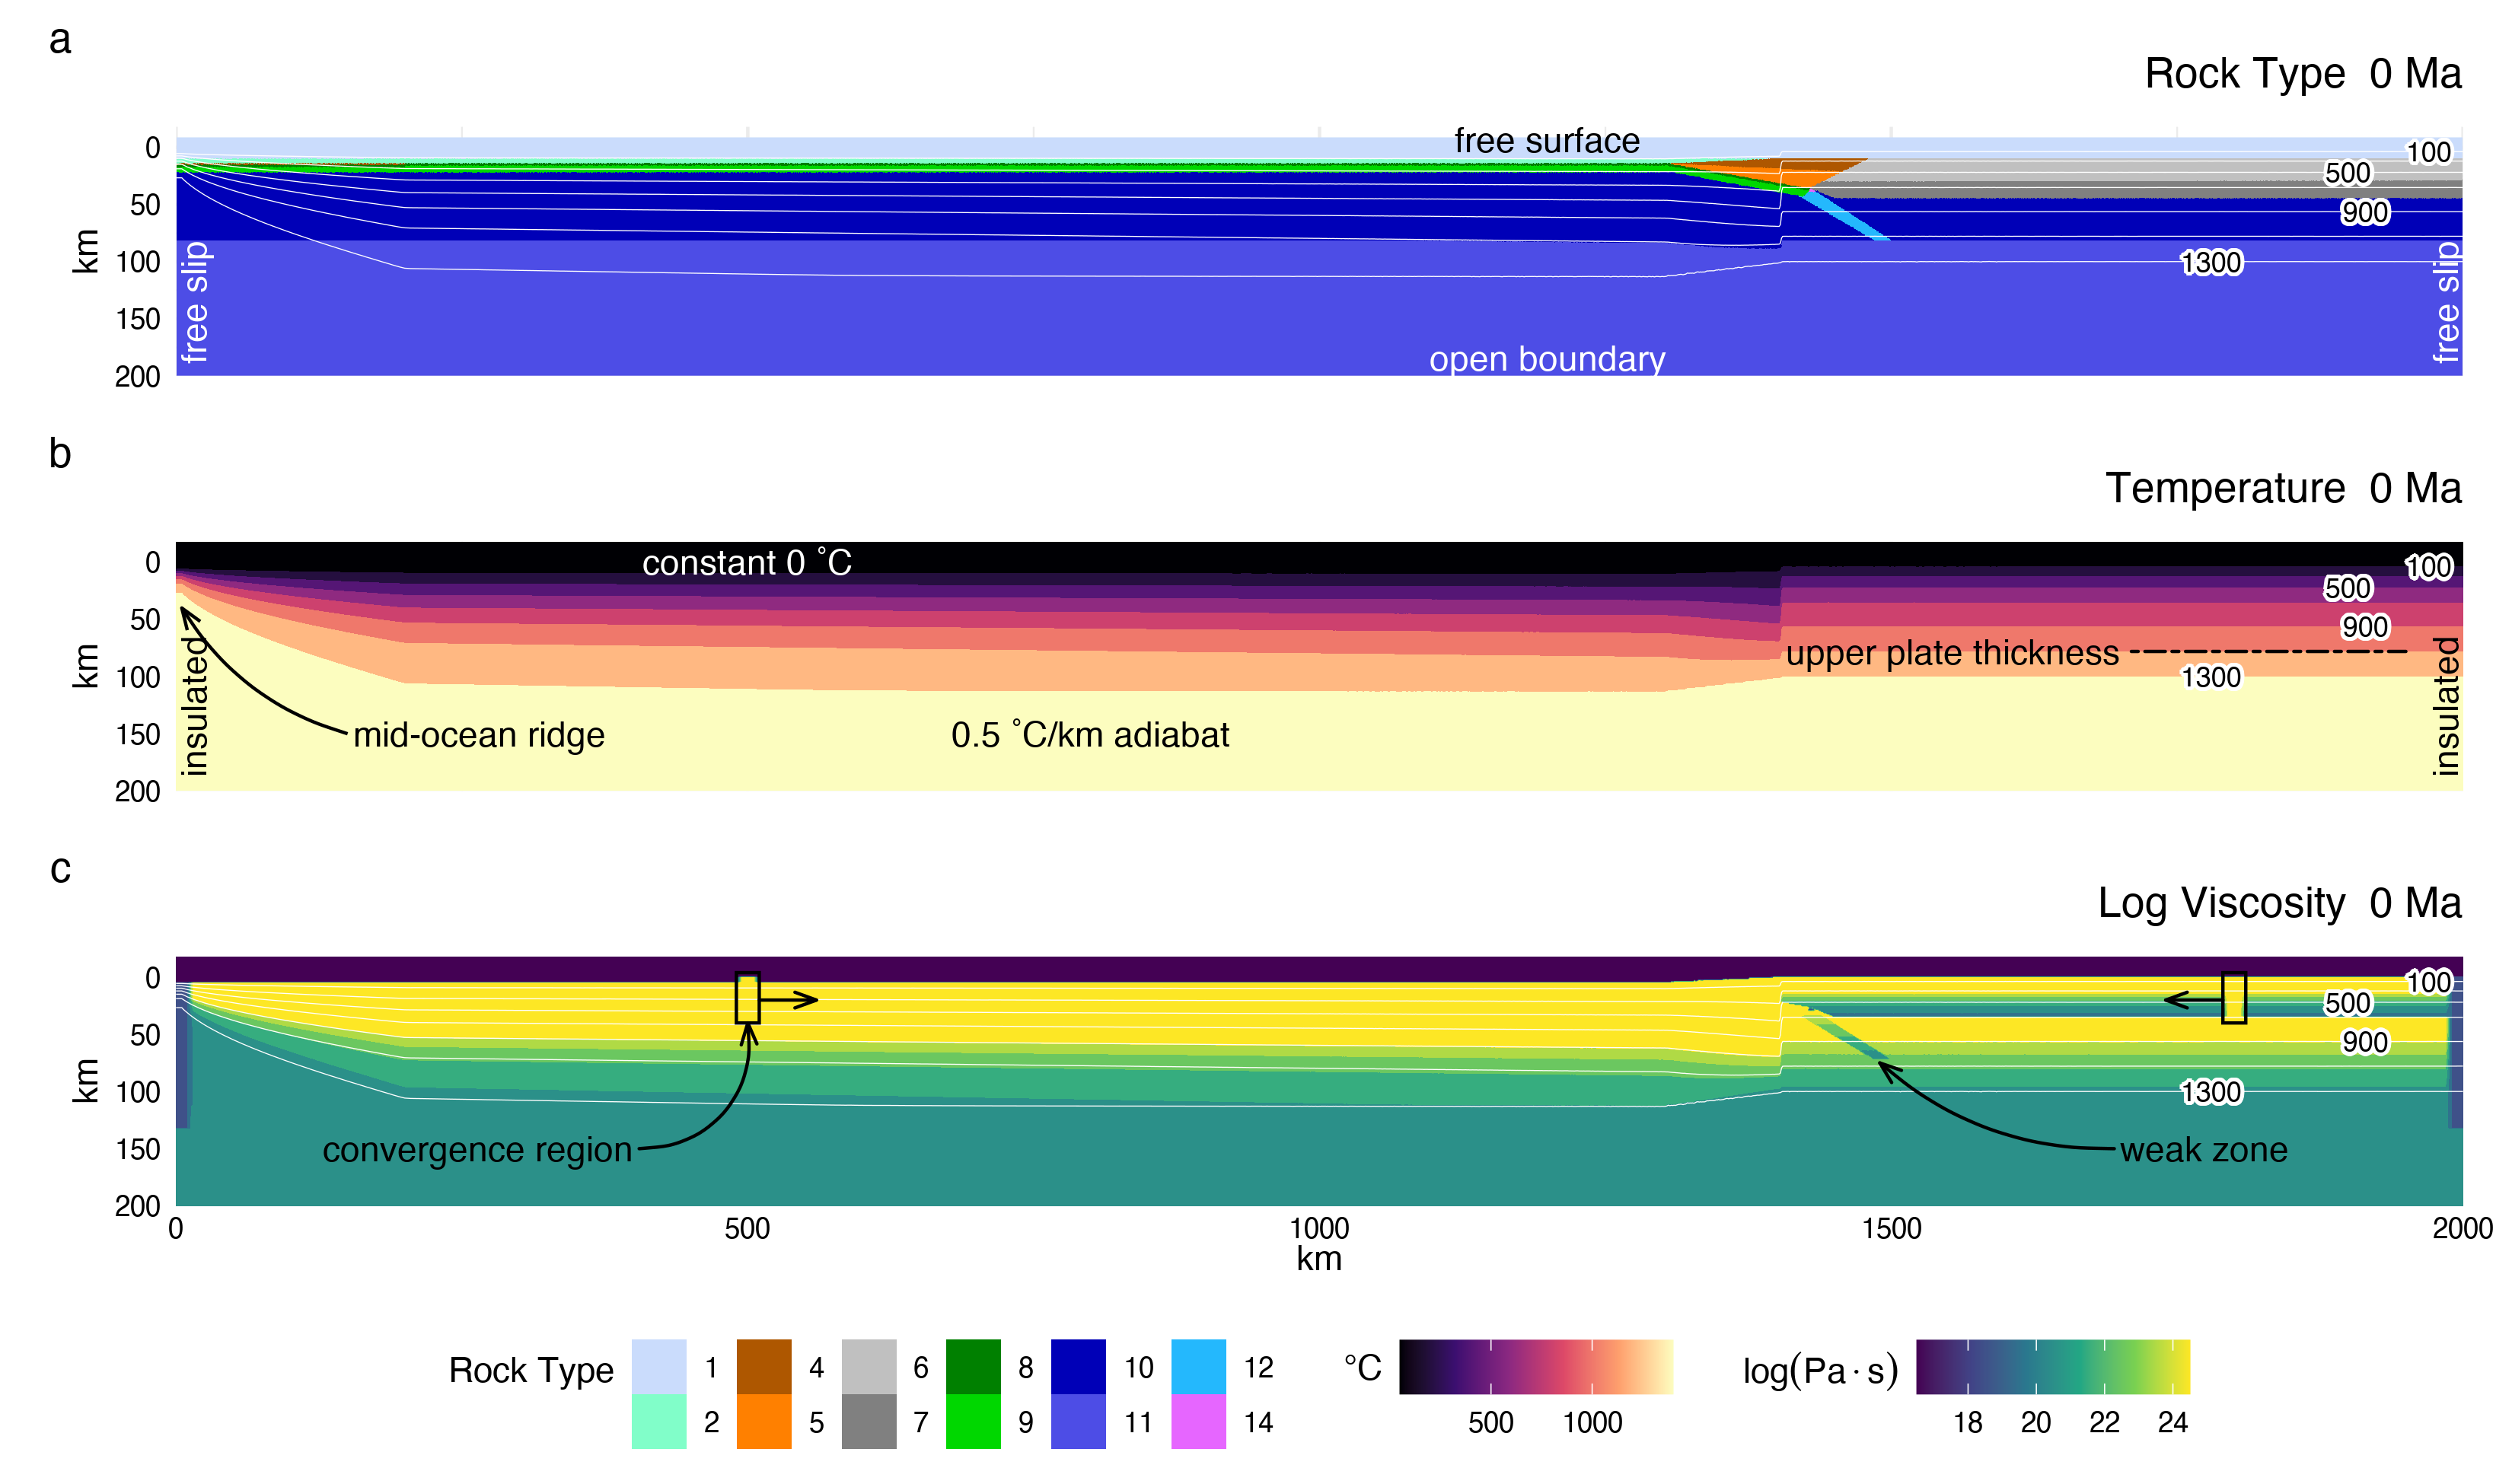
\includegraphics[width=\textwidth, trim={0 0 0 0}]{figs/Fig1.png}
 \caption{Initial model configuration and boundary conditions. (a) A free sedimentation/erosion boundary at the surface is maintained by implementing a layer of “sticky” air and water, and an infinite-like open boundary at the bottom allows for slab penetration. Oceanic lithosphere is continually created at the left boundary and convergence velocities are imposed at stationary regions far from the trench. The left and right boundaries are free slip and insulative. (b) The initial material distribution includes 7 $km$ of oceanic crust (2 $km$ basalt, 5 $km$ gabbro), 1 $km$ of oceanic sediments,  and 35 $km$ of continental crust, thinning ocean-ward. The oceanic crust is bent under loading from passive margin sediments, and a weak zone (high pore fluid pressure) extends from the deflected oceanic crust, through the lithosphere, to help induce subduction. (c) The oceanic geotherm is calculated using a half-space cooling model and the continental geotherm is calculated using a one-dimensional steady-state conductive cooling model to 1300 $^{\circ}C$. The base of the lithosphere is defined mechanically through visualization of viscosity and generally coincides with the 1100 $^{\circ}C$ isotherm ($z_{1100}$).}
 \label{Figure1}
\end{sidewaysfigure}

A horizontal convergence velocity was applied to both plates in a rectangular region far from the continental margin (Fig.~\ref{Figure1}a). A convergence force and initial weak layer (high pore fluid pressure) cutting the lithosphere permitted subduction to initiate. The rectangular convergence regions prescribed inside the plates maintained a constant viscosity of $\eta = 10^25 Pa\cdot s$ to apply constant horizontal velocities without deforming the lithosphere. The subduction angle was not prescribed and was governed by the free-motion of the sinking slab. Similarly, subduction velocity can vary with time in response to extension or shortening of the overriding plate. Therefore, we calculated the slab thermal parameter ($\Phi$) as the product of the horizontal convergence velocity ($km/Ma$) and the slab age \cite<$Ma$; c.f.>[]{McKenzie1969}.  We use $\Phi$/100 as it is commonly presented in the literature to reduce the thermal parameter to convenient figures (Fig.~\ref{Figure2}a).

\begin{figure}
 \centering
 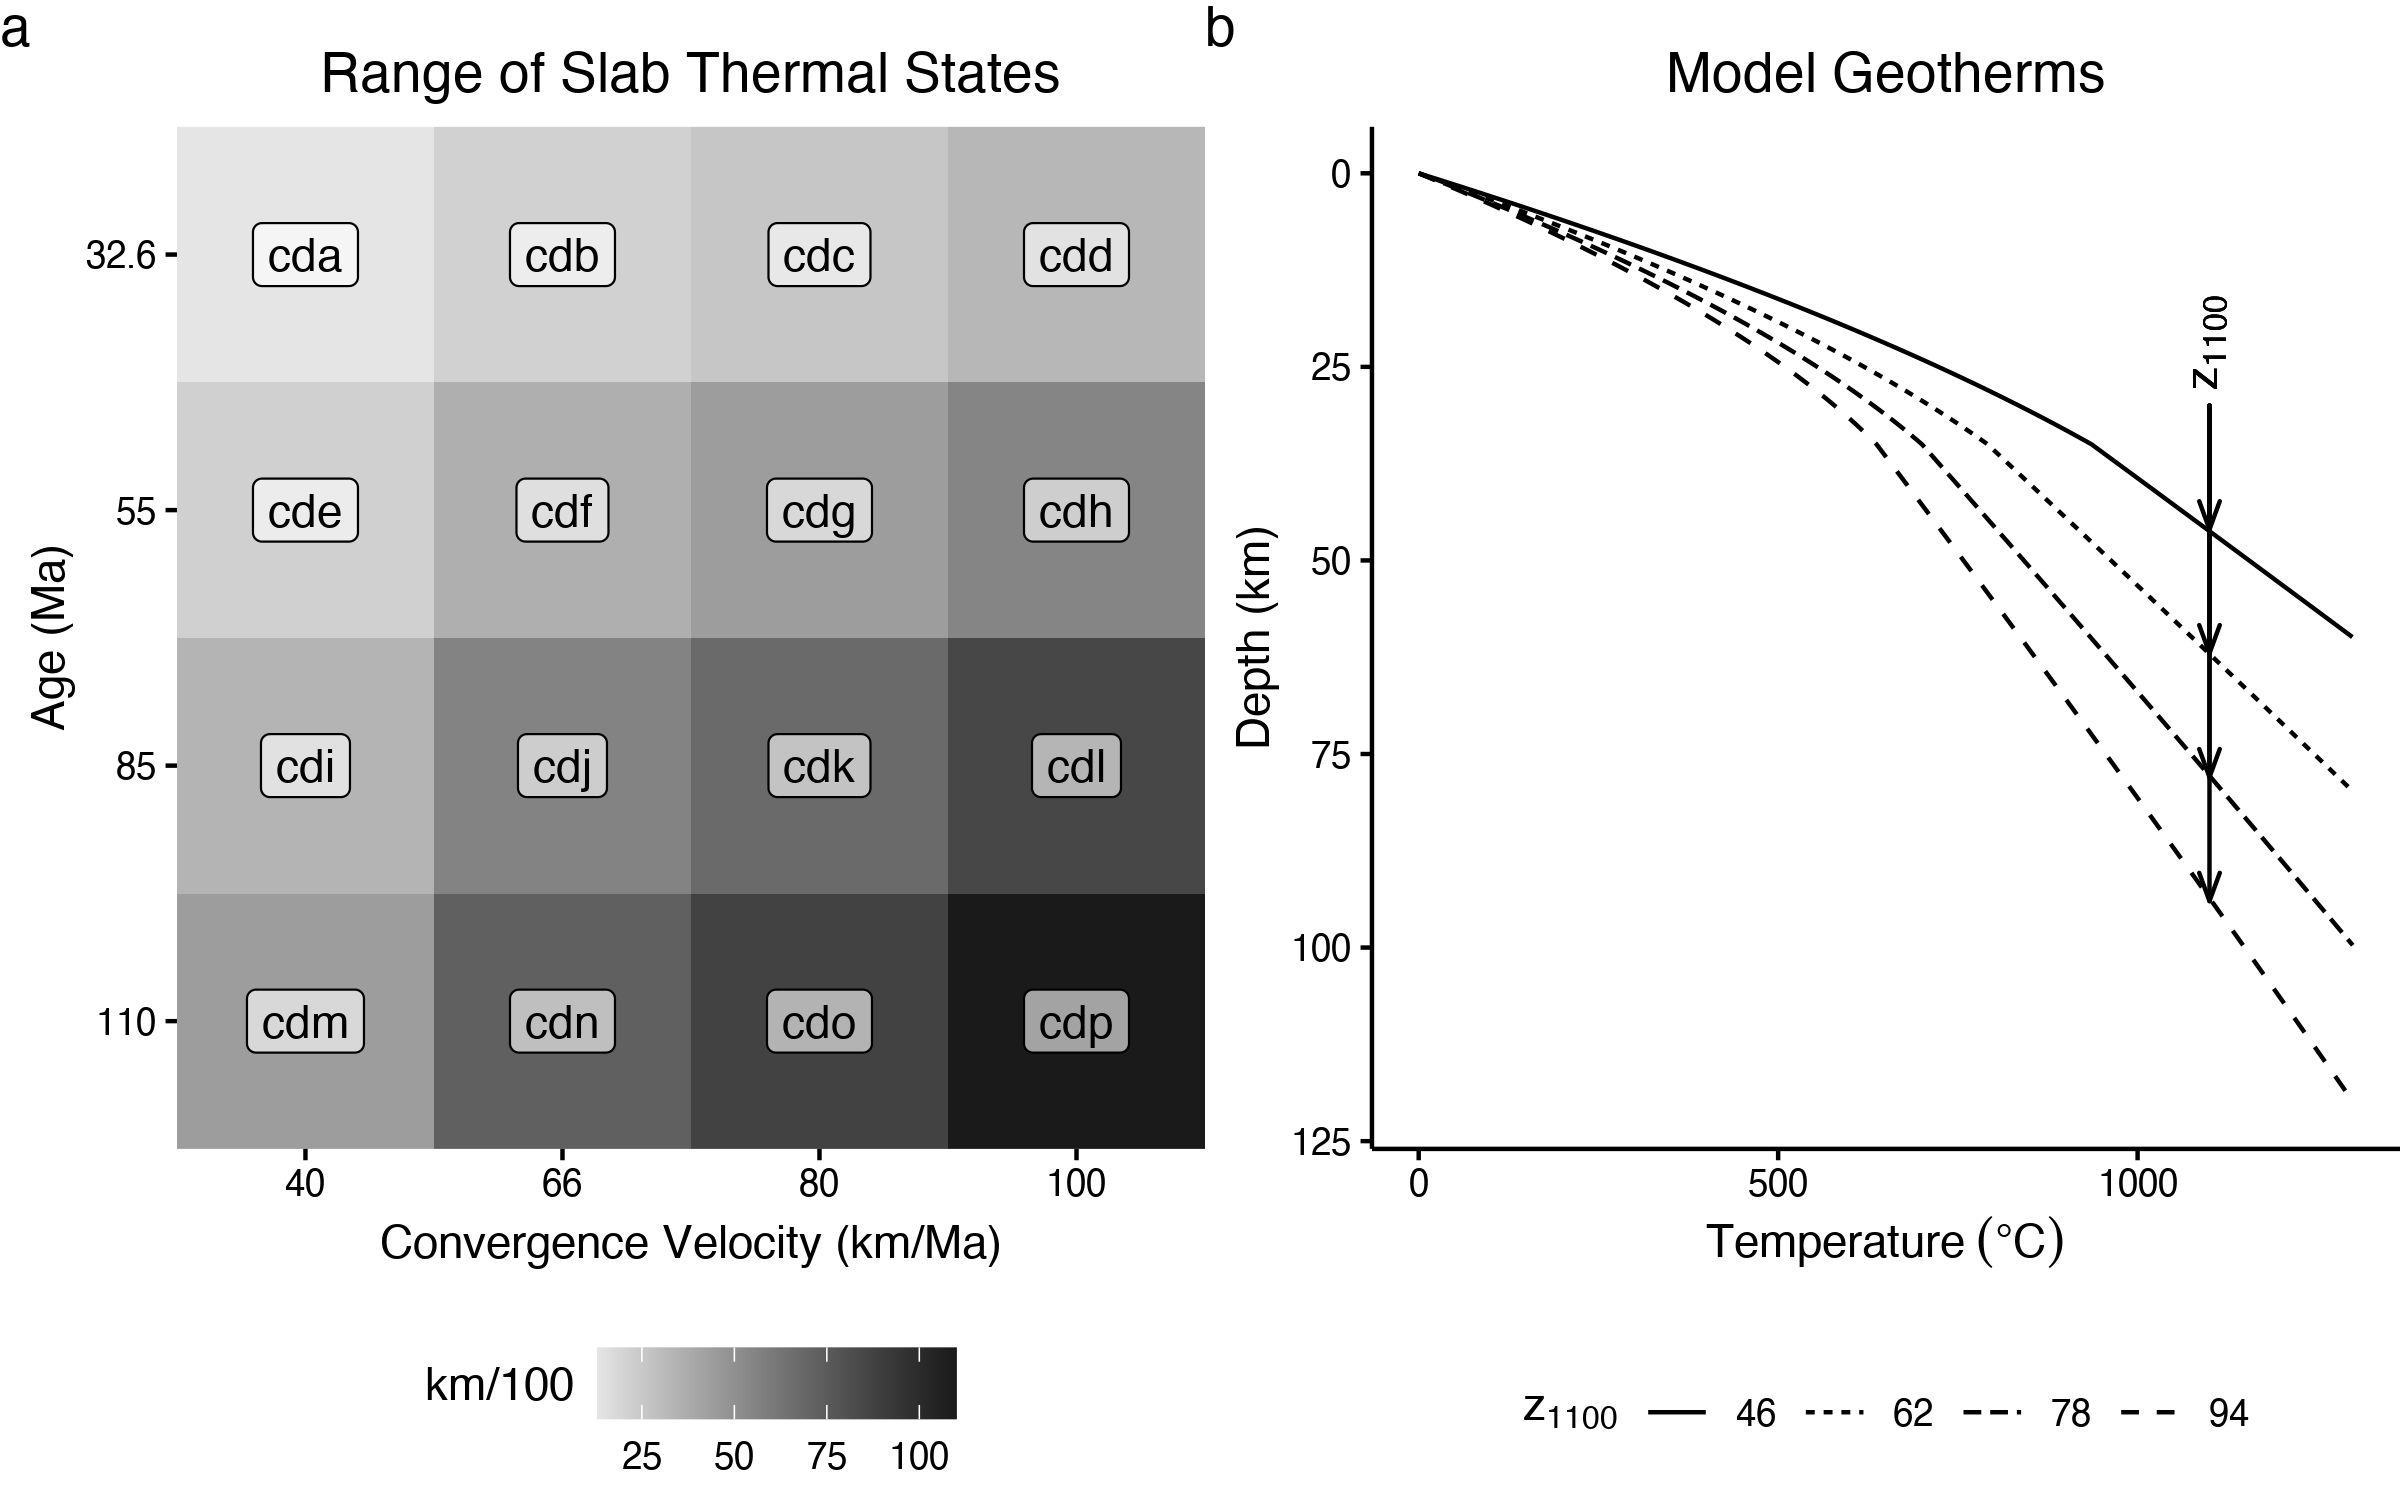
\includegraphics[width=\textwidth, trim={0 0 0 0}]{figs/Fig2.png}
 \caption{The range of key parameters investigated in this study. (a) Modelled slab ages and convergence velocities broadly reflect the middle-range of the global distribution of modern subduction zones with thermal parameters ranging from 13 to 110 $km/100$. Model names include the prefix "cd" for "coupling depth" with arbitrarily increasing alphabetic suffixes. (b) Geotherms were constructed using a one-dimensional steady-state conductive cooling model using T(z=0) = 0 $^{\circ}$C and q(z=0) = 59, 63, 69, 79 $mW/m^2$, and constant radiogenic heating of 1.0 $\mu W/m^3$ for a 35 $km$-thick crust and 0.022 $\mu W/m^3$ for the mantle. The continental geotherms are calculated up to 1300 $^{\circ}$C, with a 0.5 $^{\circ}$C/km gradient (the mantle adiabat) for higher temperatures.}
 \label{Figure2}
\end{figure}

\subsection{Calculating geotherms and defining lithospheric thickness}
The oceanic crust was modeled as 1 $km$ of sediment cover overlying 2 $km$ of basalt and 5 $km$ of gabbro (Fig.~\ref{Figure1}b). Oceanic lithosphere was continually made at a pseudo-mid-ocean ridge on the left boundary of the model and an enhanced vertical cooling condition was applied at 200 $km$ from the mid-ocean ridge to adjust for the proper oceanic plate age, and therefore its lithospheric thickness as it enters the trench \cite<Fig.~\ref{Figure1}c;>{Agrusta2013}. We used plate ages from 32.6 to 110 $Ma$ and convergence velocities from 40 to 100 $km/Ma$ (Fig.~\ref{Figure2}a). This range of slab parameters broadly reflects the middle-range of the modern global subduction system \cite{Syracuse2006}.

The initial continental geotherms were determined by solving the heat flow equation in one-dimension to 1300 $^{\circ}C$ (Fig.~\ref{Figure2}b). We assumed a fixed temperature of 0 $^{\circ}C$ at the surface, constant radiogenic heating of 1 $\mu W/m^3$ in the 35 $km$-thick continental crust and 0.022 $\mu W/m^3$ in the mantle, and thermal conductivities of 2.3 $W/mK$ and 3.0 $W/mK$ for the continental crust and mantle, respectively. Below the 1300 $^{\circ}C$ isotherm the temperature increases by 0.5 $^{\circ}C/km$ (the mantle adiabat).

Many studies define the base of the continental lithosphere at the 1300 $^{\circ}C$ isotherm, but it can be determined more accurately from viscosity and strain rate as the model progresses. The mechanical base of the lithosphere in our models generally occurred around the 1100 $^{\circ}C$ isotherm\textemdash characterized by a rapid decrease in viscosity and increase in strain rate. As such, we consider the oceanic and continental lithosphere in this study as mechanical layers. For convenience, we refer to the continental lithospheric thickness as $z_{1100}$ because its correspondence with the 1100 $^{\circ}C$ isotherm makes it discernable in figures where we draw isotherms, but do not explicitly visualize viscosity or strain rate. To match our modelled range of backarc heat flow, $z_{1100}$ ranged from 46 to 94 $km$ (Fig.~\ref{Figure2}b).

\subsection{Metamorphic (de)hydration reactions}
Our use of Lagrangian markers to store pressure, temperature, and rheology corresponding with rock-specific flow laws allows for changes to material properties (e.g., viscosity, density, etc.) that can result from metamorphic reactions. In our models, we focused on dehydration reactions in the slab and the formation and breakdown of antigorite in the mantle wedge. For computational efficiency our models did not solve for thermodynamically stable mineral assemblages to compute water contents for the slab and mantle wedge \cite<e.g.,>[]{Connolly2005}. Instead, for the slab, we implemented a simple model for gradual dehydration (eclogitization) of the crust computed as a linear function of depth (lithostatic pressure) with a maximum depth (150 $km$) where the slab was completely dehydrated. This approach effectively simulates a continuous influx of water to the mantle wedge, beginning with compaction and release of connate water at shallow depths, followed by a sequence of reactions consuming major hydrous phases (chlorite, lawsonite, zoisite, chloritoid, talc, amphibole, and phengite) in different parts of the hydrated basaltic crust \cite{Schmidt1998}.

For the mantle wedge, hydration of strong peridotite to form weak brucite and serpentine along the subduction interface is likely responsible for mechanical decoupling between the slab and the mantle wedge at shallow levels \cite{Peacock1999a, Hyndman2003}. If so, noting that brucite breaks down at much lower temperatures than serpentine \cite{Schmidt1998}, the loss of serpentine likely represents the key transition from a weak wedge (and subduction interface) to a strong wedge. Dehydration of serpentine was modelled as an abrupt, discontinuous reaction, which is a good approximation for extremely Mg-rich rocks like peridotites. The P-T conditions of the reaction $antigorite \Leftrightarrow olivine + orthopyroxene + H_{2}O$ were based on the experimentally determined stability field from \citeA{Schmidt1998} and implemented into our model using the following equation:

\begin{equation}
 \begin{alignedat}{2}
  T_{atg-out}(z) &= 751.50+\num{6.008d-3}z-\num{3.469d-8}z^2, && \text{for $z<63000m$} \\
  T_{atg-out}(z) &= 1013.2-\num{6.039d-5}z-\num{4.289d-9}z^2, && \text{for $z>63000m$}
 \end{alignedat}
 \label{Equation1}
\end{equation}

where $z$ is the depth of a marker from the surface in meters and $T$ is temperature in Kelvins. This reaction placement is also consistent to within 25 $^{\circ}C$ with recent experiments \cite{Shen2015}. Under assumptions of thermodynamic equilibrium, markers whose internal temperature exceeds $T(z)$  spontaneously formed $olivine \allowbreak+ orthopyroxene \allowbreak+ H_2O$, releasing their crystal-bound water.

The excess water released by a rock marker was modelled as a fluid particle that migrates through rocks with a velocity defined by pressure gradients \cite[see Appendix A]{Faccenda2009}. The fluid particle migrates until it reaches material that can consume an additional amount of water by equilibrium  hydration reactions (e.g., equation~\ref{Equation1}). Theoretically, the mantle can store large amounts of water because antigorite is stable at shallow mantle conditions and can contain up to 13 $wt.\%$ water \cite{Reynard2013}. Thermodynamic models predict 8 $wt.\%$ water in the mantle wedge \cite{Connolly2005}. However, seismic studies suggest that most forearcs are only partially serpentinized ($<$ 20-40 $\%$), equating to water contents of ca. 3-6 $wt.\%$ \cite{Abers2017, Carlson2003}. Therefore we limit mantle wedge hydration to $\leq$ 2 $wt.\% ~H_2O$ and assume any $H_2O$ in excess exits the system through channelized fluid flow \cite{Davies1999}.

\subsection{Calculating surface heat flow}
We calculated vertical heat flux based on the temperature difference between the 2 $km$ deep node and the next lower node, their separation distance, and the average thermal conductivity between them. We calculated heat flux at 2 $km$ depth rather than at the surface to avoid numerical errors.

\subsection{Visualization and determination of coupling depth}
For each run (e.g., Fig.~\ref{Figure3}) we made calculations at $\sim$10 $Ma$ for surface heat flow (Fig.~\ref{Figure3}a) and visualized rock type (Fig.~\ref{Figure3}b, c), temperature (Fig.~\ref{Figure3}d), viscosity (Fig.~\ref{Figure3}e), strain rate (Fig.~\ref{Figure3}f), and an effective P\'{e}clet number (detailed below). We chose 10 $Ma$ because changes to the overall dynamics and thermal structure are small after ca. 5 $Ma$ and the additional 5 $Ma$ provides sufficient time for the geodynamics to fully stabilize (see Fig.~\ref{FigureS1}).

\begin{center}
 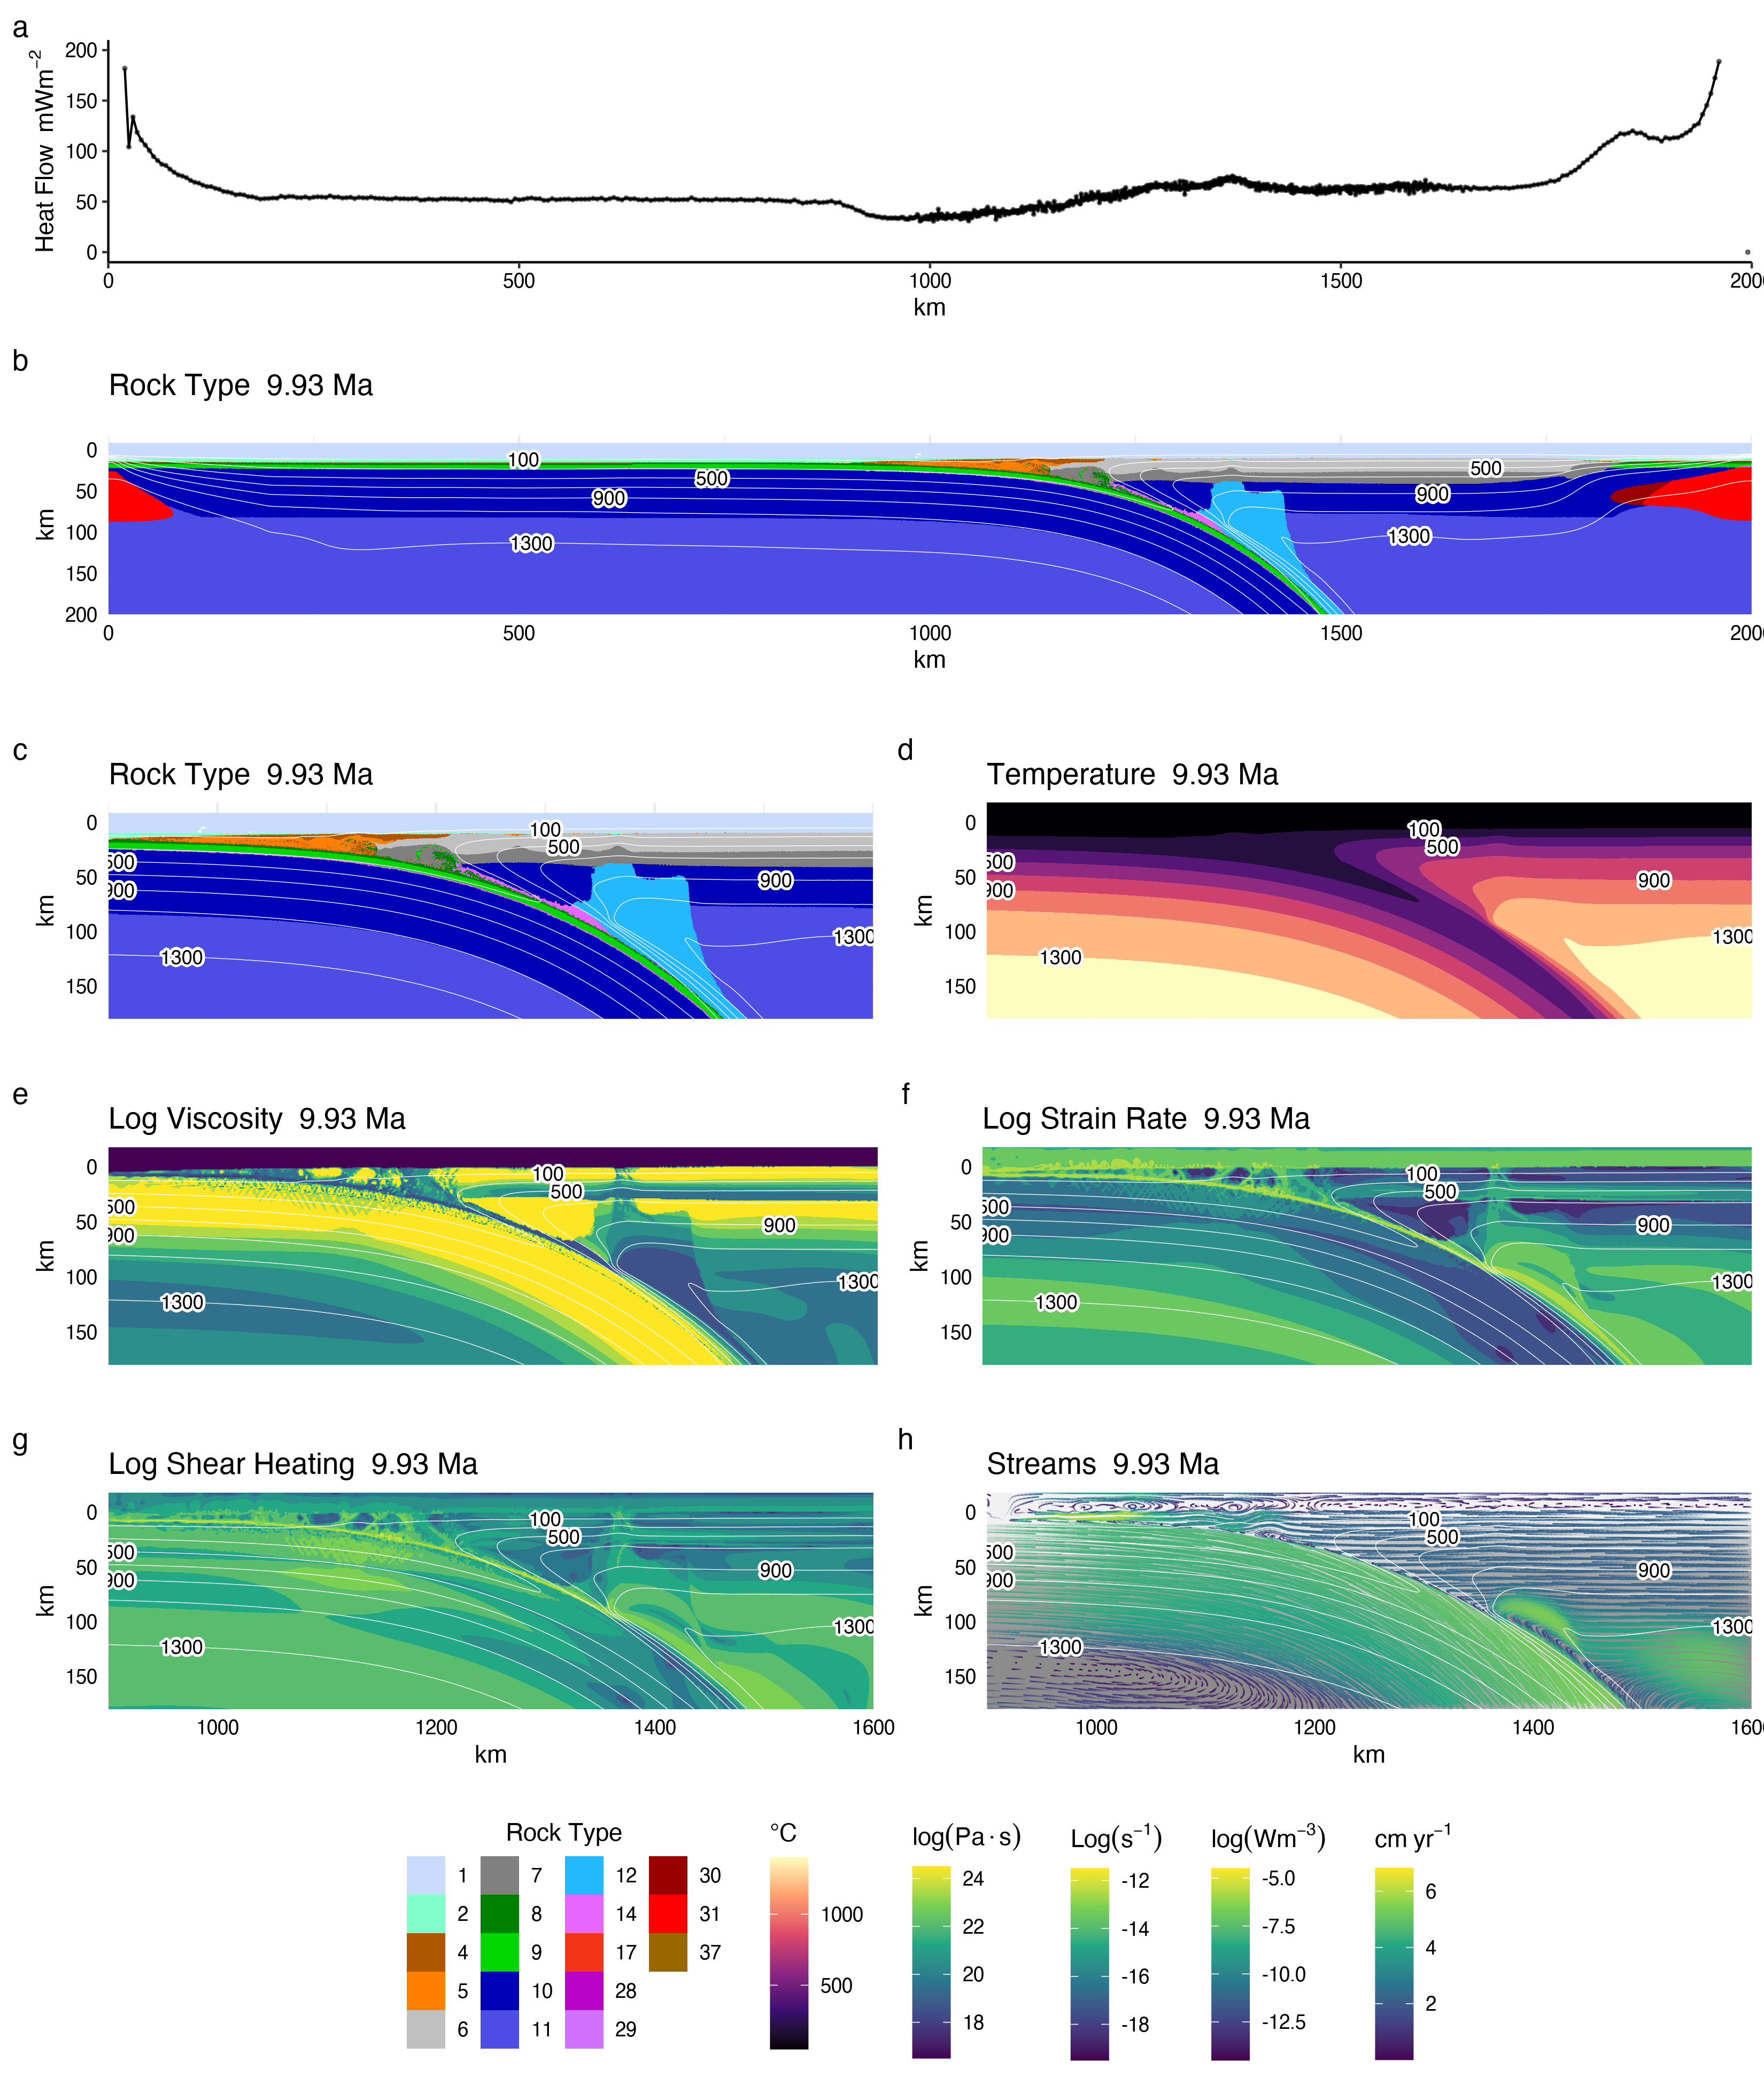
\includegraphics[width=\textwidth, trim={0 0 0 0}]{figs/Fig3.png}
 \label{Figure3}
 \captionof{figure}{Visualization of model cdf with a 78 $km$-thick backarc lithosphere at $\sim$10 $Ma$. Arc positions are marked by triangles. (a) Surface heat flow calculated at a depth of 2 $km$ beneath the surface(see text for explanation). (b) Rock type for the entire model domain. (c) Rock type in the region from the trench to approximately 220 $km$ into the backarc. By 10 $Ma$ a serpentine channel has formed, entraining material from the top of the down-going slab and lubricating the interface between slab and mantle. (d) Temperature distribution. (e) Log viscosity. The viscosity contrast between the slab and serpentinized mantle in the forearc effectively decouples the slab and mantle wedge mechanically, but abruptly diminishes as the principally weak material (antigorite) is removed by reaction. (f) Log strain rate. In the shallow forearc, strain is localized in the weak serpentine channel. At the antigorite-out reaction, strain localization jumps towards the warm core of the mantle wedge. Circulation in the mantle wedge is restricted to beneath the stiff lithosphere. (g) Effective P\'{e}clet number. An effective P\'{e}clet number is the ratio of advective:conductive heat transport, scaled to the local thermal gradients (see text for formulation). “Cooler” colors (blues) vs. “warmer” colors (reds) indicate advection up vs. down the thermal gradient, i.e., high values show advection in the same direction as diffusion. An absolute value between 0 and ~10 (green) indicates much greater efficiency of heat transfer via thermal diffusion than via advection, whereas absolute values greater than ~40 (blues and reds) indicate high efficiency of heat transfer via advection \textit{and/or} a small local thermal gradient. Note the narrow region of dark red streaming towards the coupling point, indicating high efficiency of heat advection into the coupling region.}
\end{center}

We determined the mechanical coupling depth ($z_c$) by visualizing viscosity at $\sim$10 $Ma$ and selecting a node closest to the point where the viscosity contrast between the serpentinized- and non-serpentinized basal mantle wedge diminishes to $<$ 10$^2$ $Pa\cdot s$ (Fig.~\allowbreak\ref{Figure3}e). In this study we assume that the mechanical coupling depth occurs instantaneously and at a single node. However, mechanical coupling in reality must be dispersed across a finite length along the slab-mantle interface. At the resolution of our models, there was a small area (ca. 5x5 $km$ or 5x5 nodes) where $z_c$ could appropriately be determined, giving an uncertainty in our $z_c$ determination on the order of $\pm$ 2.5 $km$.

\subsection{Formulation of an effective P\'{e}clet number}
We calculated what we call the “effective P\'{e}clet number” to visualize and evaluate potential thermal feedbacks affecting the stability of antigorite in the mantle wedge. In its normal formulation, the P\'{e}clet number is a dimensionless number used to visualize the relative magnitude of (potential) heat transfer via advection vs. diffusion in a continuum \cite{Patankar2018}:

\begin{equation}
 \begin{gathered}
  Pe=\frac{advective~transport~rate}{diffusive~transport~rate} \\
  Pe=\frac{Lv}{\alpha} \\
  \alpha=\frac{\kappa}{\rho c_p}
 \end{gathered}
 \label{Equation3}
\end{equation}

where $L$ is a characteristic length, $v$ is the local velocity of the continuum, $\alpha$ is thermal diffusivity (or thermal diffusion coefficient), $\kappa$ is thermal conductivity, $\rho$ is the density, and $c_p$ is specific heat capacity.

It is important to recognize that equation~\ref{Equation3} makes no explicit reference to the direction of heat transport. In particular, while heat always conducts down the (maximum) temperature gradient, i.e., perpendicular to isotherms and from high temperature to low temperature, advection may occur in any direction. Thus, depending on flow paths, advection could (a) augment local heat transport (a component of flow is parallel to and in the same direction as diffusion), (b) retard local heat transport (a component of flow is parallel to but in the opposite direction as diffusion) or (c) have no effect on local heat transport (flow is parallel to isotherms).

In regions of complex flow dynamics and thermal structure, the standard formulation of the P\'{e}clet number can lead to implausible interpretations. For example, below the coupling depth, the base of the mantle wedge cools and new lithosphere forms atop the slab, which is dragged down by slab motion (Fig.~\ref{Figure3}e, g). This region has a high P\'{e}clet number, as calculated by equation~\ref{Equation3}, because the local velocity is very high and the thermal diffusion coefficient is only moderate. This form of the P\'{e}clet number would imply that thermal advection dominates heat transport. However, the closely spaced isotherms (large temperature gradients) within the same region imply that thermal diffusion is highly effective at transporting heat (Fig.~\ref{Figure3}g), while flow paths are nearly parallel to isotherms, implying that advection is ineffective. In terms of the effectiveness of heat transport, diffusion strongly outweighs advection, so intuitively the P\'{e}clet number should be small, not large.

To better characterize heat transfer, we scale the P\'{e}clet number to the local thermal gradients as follows:

\begin{equation}
 Pe=\frac{Lv\nabla T_v}{\alpha\nabla T_{max}}
 \label{Equation4}
\end{equation}

where $\nabla T_v$ is the local thermal gradient \protect\textit{in the direction of the local velocity field}, and $\nabla T_{max}$ is the maximum local thermal gradient that defines the effectiveness of heat diffusion. This formulation gives a better sense of heat transfer in a system where thermal gradients and velocity fields are highly non-uniform and have high contrasts. For the characteristic length scale, $L$, we use the slab thermal parameter, which scales the expression to the convergence velocity of the slab and the slab age, conveniently yielding numbers between 0 and 100 in most models. The final expression becomes:

\begin{equation}
 Pe=\frac{\Phi v\nabla T_v}{\alpha\nabla T_{max}}
 \label{Equation5}
\end{equation}

Because the temperature gradient in the direction of local flow can be positive or negative, an effective P\'{e}clet number can be positive or negative, where negative values indicate that advection and diffusion operate in opposite directions.

\section{Results}
\subsection{Coupling depth predictors}
Across all 64 numerical models (Fig.~\ref{Figure4}; Table~\ref{Table3}) coupling depth correlates strongly, but not linearly, with increasing backarc lithospheric thickness ($z_{1100}$; Fig.~\ref{Figure5}a). This correlation is a key result of our experiments. Slab thermal parameter alone does not correlate obviously with coupling depth (Fig.~\ref{Figure5}b). We determined the best fit model by considering standard least squares regressions that include all possible permutations of the variables $z_{1100}$, $z_{1100}^2$, and $\Phi$ (Tables~\ref{TableS1} and \ref{TableS2}):

\begin{equation}
 z_{coupling}\sim \num{4.95d-3}z_{1100}^2-\num{9.27d-2}\Phi+63.6
 \label{Equation6}
\end{equation}

where $z$ and $\Phi$ are in $km$. Equation~\ref{Equation6} permits the prediction of the mechanical coupling depths in modern subduction zones where backarc lithospheric thickness (inverted from backarc heat flow) and slab thermal parameter can be estimated. A web-based application to perform such calculations is available for free online (see Appendix A)

\begin{figure}
 \centering
 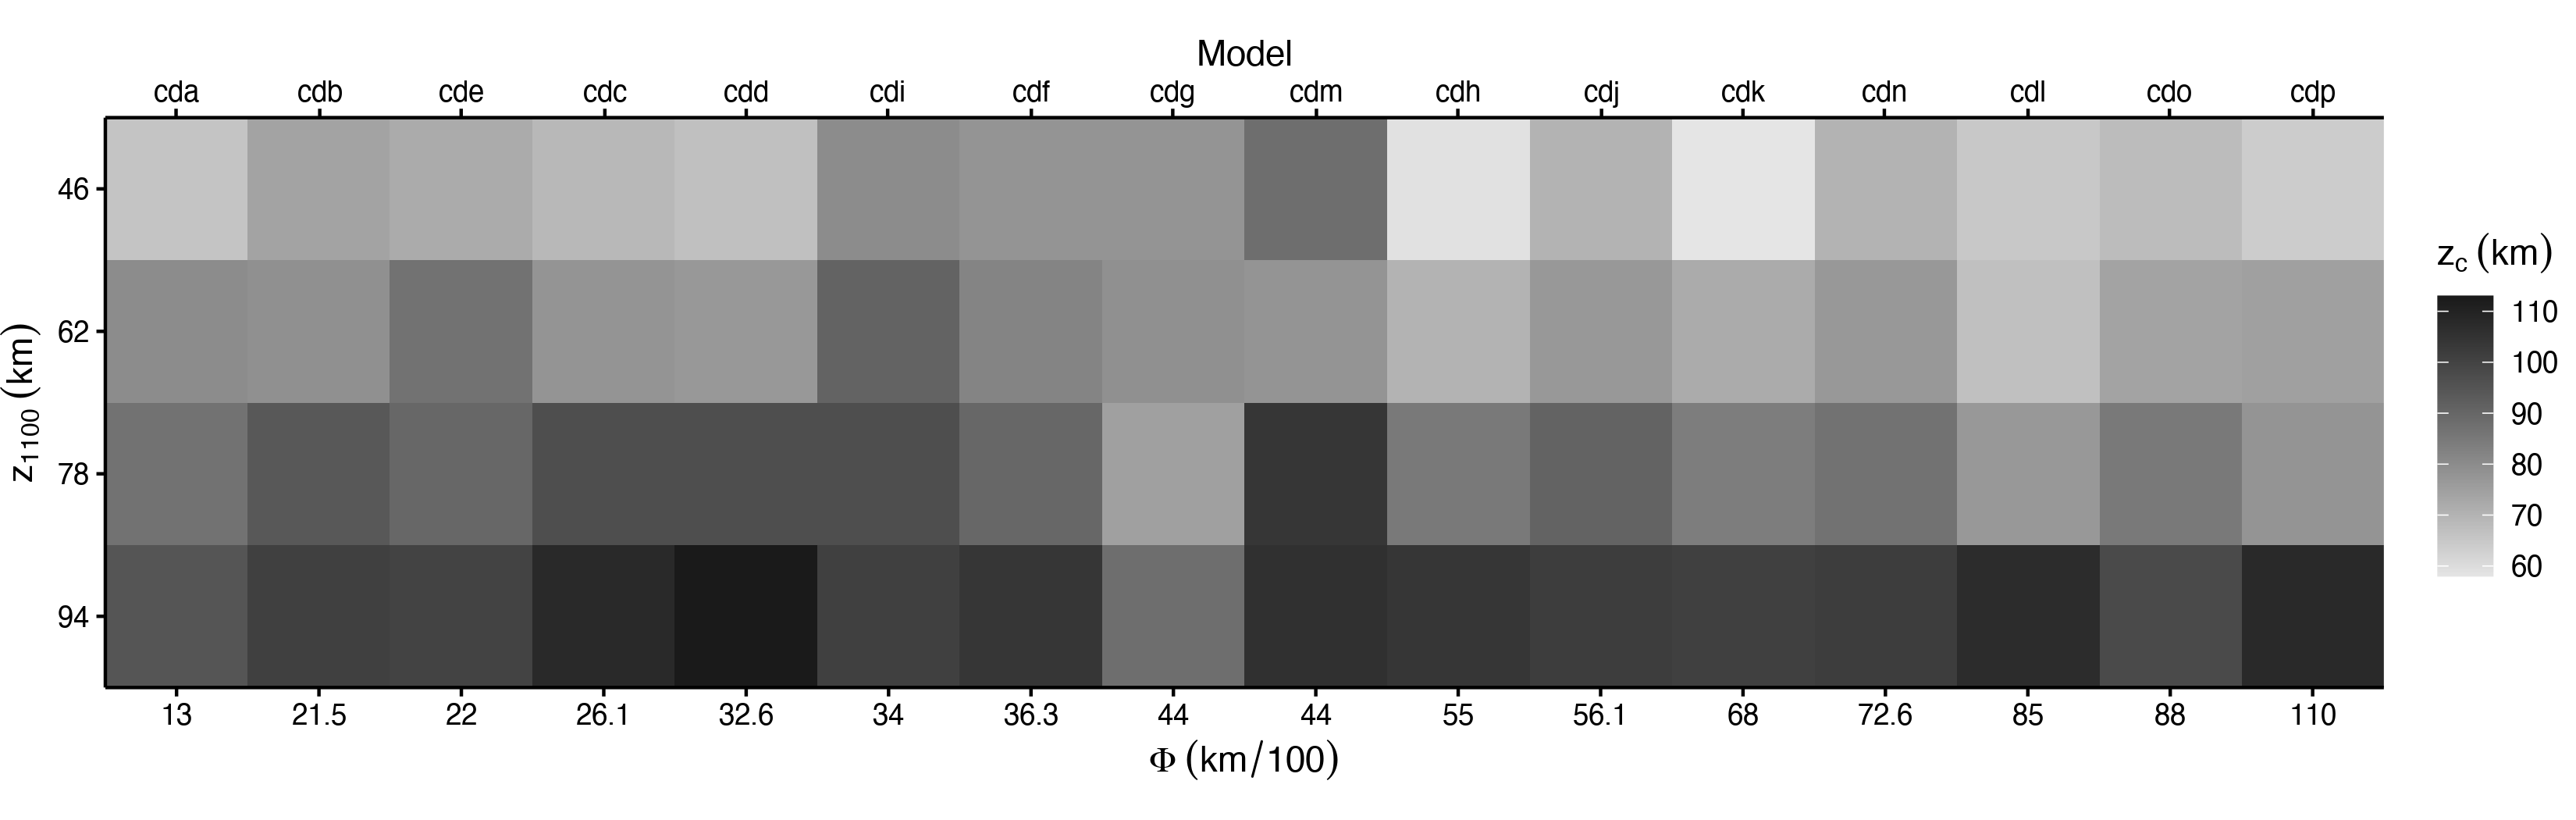
\includegraphics[width=\textwidth, trim={0 0 0 0}]{figs/Fig4.png}
 \caption{Visualized table of coupling depth as determined across a range of lithospheric thicknesses and thermal parameters. Note that the thermal parameter axis is not linear. Corresponding experiment is listed along the top of the array. Coupling depth increases systematically with increasing backarc lithospheric thickness (change in grayscale down columns) for all models. Any trend in coupling depth with respect to slab thermal parameter (change in grayscale across rows) is not apparent.}
 \label{Figure4}
\end{figure}

\begin{longtable}{A{0.13} B{0.12} B{0.12} B{0.10}}
 \caption{Experimental results}               \\
 \label{Table3}                               \\
 \toprule

 Experiment & $z_{1100}$ & $\phi/100$ & $z_c$ \\
            & $km$       & $km/100$   & $km$  \\

 \midrule
 \endfirsthead

 \caption{Experimental results (cont.).}      \\
 \label{Table3}                               \\
 \toprule

 Experiment & $z_{1100}$ & $\phi/100$ & $z_c$ \\
            & $km$       & $km/100$   & $km$  \\

 \midrule
 \endhead

 \midrule
 \multicolumn{4}{r}{\footnotesize Continued on the next page}
 \endfoot
 \bottomrule
 \endlastfoot

 cda        & 46         & 13.0       & 66    \\
 cdb        & 46         & 21.5       & 74    \\
 cdc        & 46         & 26.1       & 69    \\
 cdd        & 46         & 32.6       & 67    \\
 cde        & 46         & 22.0       & 72    \\
 cdf        & 46         & 36.3       & 78    \\
 cdg        & 46         & 44.0       & 78    \\
 cdh        & 46         & 55.0       & 59    \\
 cdi        & 46         & 34.0       & 80    \\
 cdj        & 46         & 56.1       & 70    \\
 cdk        & 46         & 68.0       & 58    \\
 cdl        & 46         & 85.0       & 65    \\
 cdm        & 46         & 44.0       & 79    \\
 cdn        & 46         & 72.6       & 70    \\
 cdo        & 46         & 88.0       & 68    \\
 cdp        & 46         & 110        & 64    \\
 cda        & 62         & 13.0       & 80    \\
 cdb        & 62         & 21.5       & 79    \\
 cdc        & 62         & 26.1       & 78    \\
 cdd        & 62         & 32.6       & 77    \\
 cde        & 62         & 22.0       & 87    \\
 cdf        & 62         & 36.3       & 82    \\
 cdg        & 62         & 44.0       & 75    \\
 cdh        & 62         & 55.0       & 70    \\
 cdi        & 62         & 34.0       & 91    \\
 cdj        & 62         & 56.1       & 77    \\
 cdk        & 62         & 68.0       & 72    \\
 cdl        & 62         & 85.0       & 67    \\
 cdm        & 62         & 44.0       & 88    \\
 cdn        & 62         & 72.6       & 77    \\
 cdo        & 62         & 88.0       & 74    \\
 cdp        & 62         & 110        & 75    \\
 cda        & 78         & 13.0       & 87    \\
 cdb        & 78         & 21.5       & 94    \\
 cdc        & 78         & 26.1       & 97    \\
 cdd        & 78         & 32.6       & 97    \\
 cde        & 78         & 22.0       & 90    \\
 cdf        & 78         & 36.3       & 90    \\
 cdg        & 78         & 44.0       & 88    \\
 cdh        & 78         & 55.0       & 85    \\
 cdi        & 78         & 34.0       & 97    \\
 cdj        & 78         & 56.1       & 91    \\
 cdk        & 78         & 68.0       & 84    \\
 cdl        & 78         & 85.0       & 77    \\
 cdm        & 78         & 44.0       & 78    \\
 cdn        & 78         & 72.6       & 87    \\
 cdo        & 78         & 88.0       & 85    \\
 cdp        & 78         & 110        & 78    \\
 cda        & 94         & 13.0       & 95    \\
 cdb        & 94         & 21.5       & 101   \\
 cdc        & 94         & 26.1       & 108   \\
 cdd        & 94         & 32.6       & 113   \\
 cde        & 94         & 22.0       & 100   \\
 cdf        & 94         & 36.3       & 104   \\
 cdg        & 94         & 44.0       & 104   \\
 cdh        & 94         & 55.0       & 104   \\
 cdi        & 94         & 34.0       & 101   \\
 cdj        & 94         & 56.1       & 102   \\
 cdk        & 94         & 68.0       & 101   \\
 cdl        & 94         & 85.0       & 107   \\
 cdm        & 94         & 44.0       & 106   \\
 cdn        & 94         & 72.6       & 102   \\
 cdo        & 94         & 88.0       & 98    \\
 cdp        & 94         & 110        & 108   \\
\end{longtable}
\begin{tablenotes}
 \footnotesize
 \item [] $z_{1100}$=lithospheric thickness, $\phi$=thermal parameter, $z_c$=coupling depth
\end{tablenotes}

\begin{figure}
 \centering
 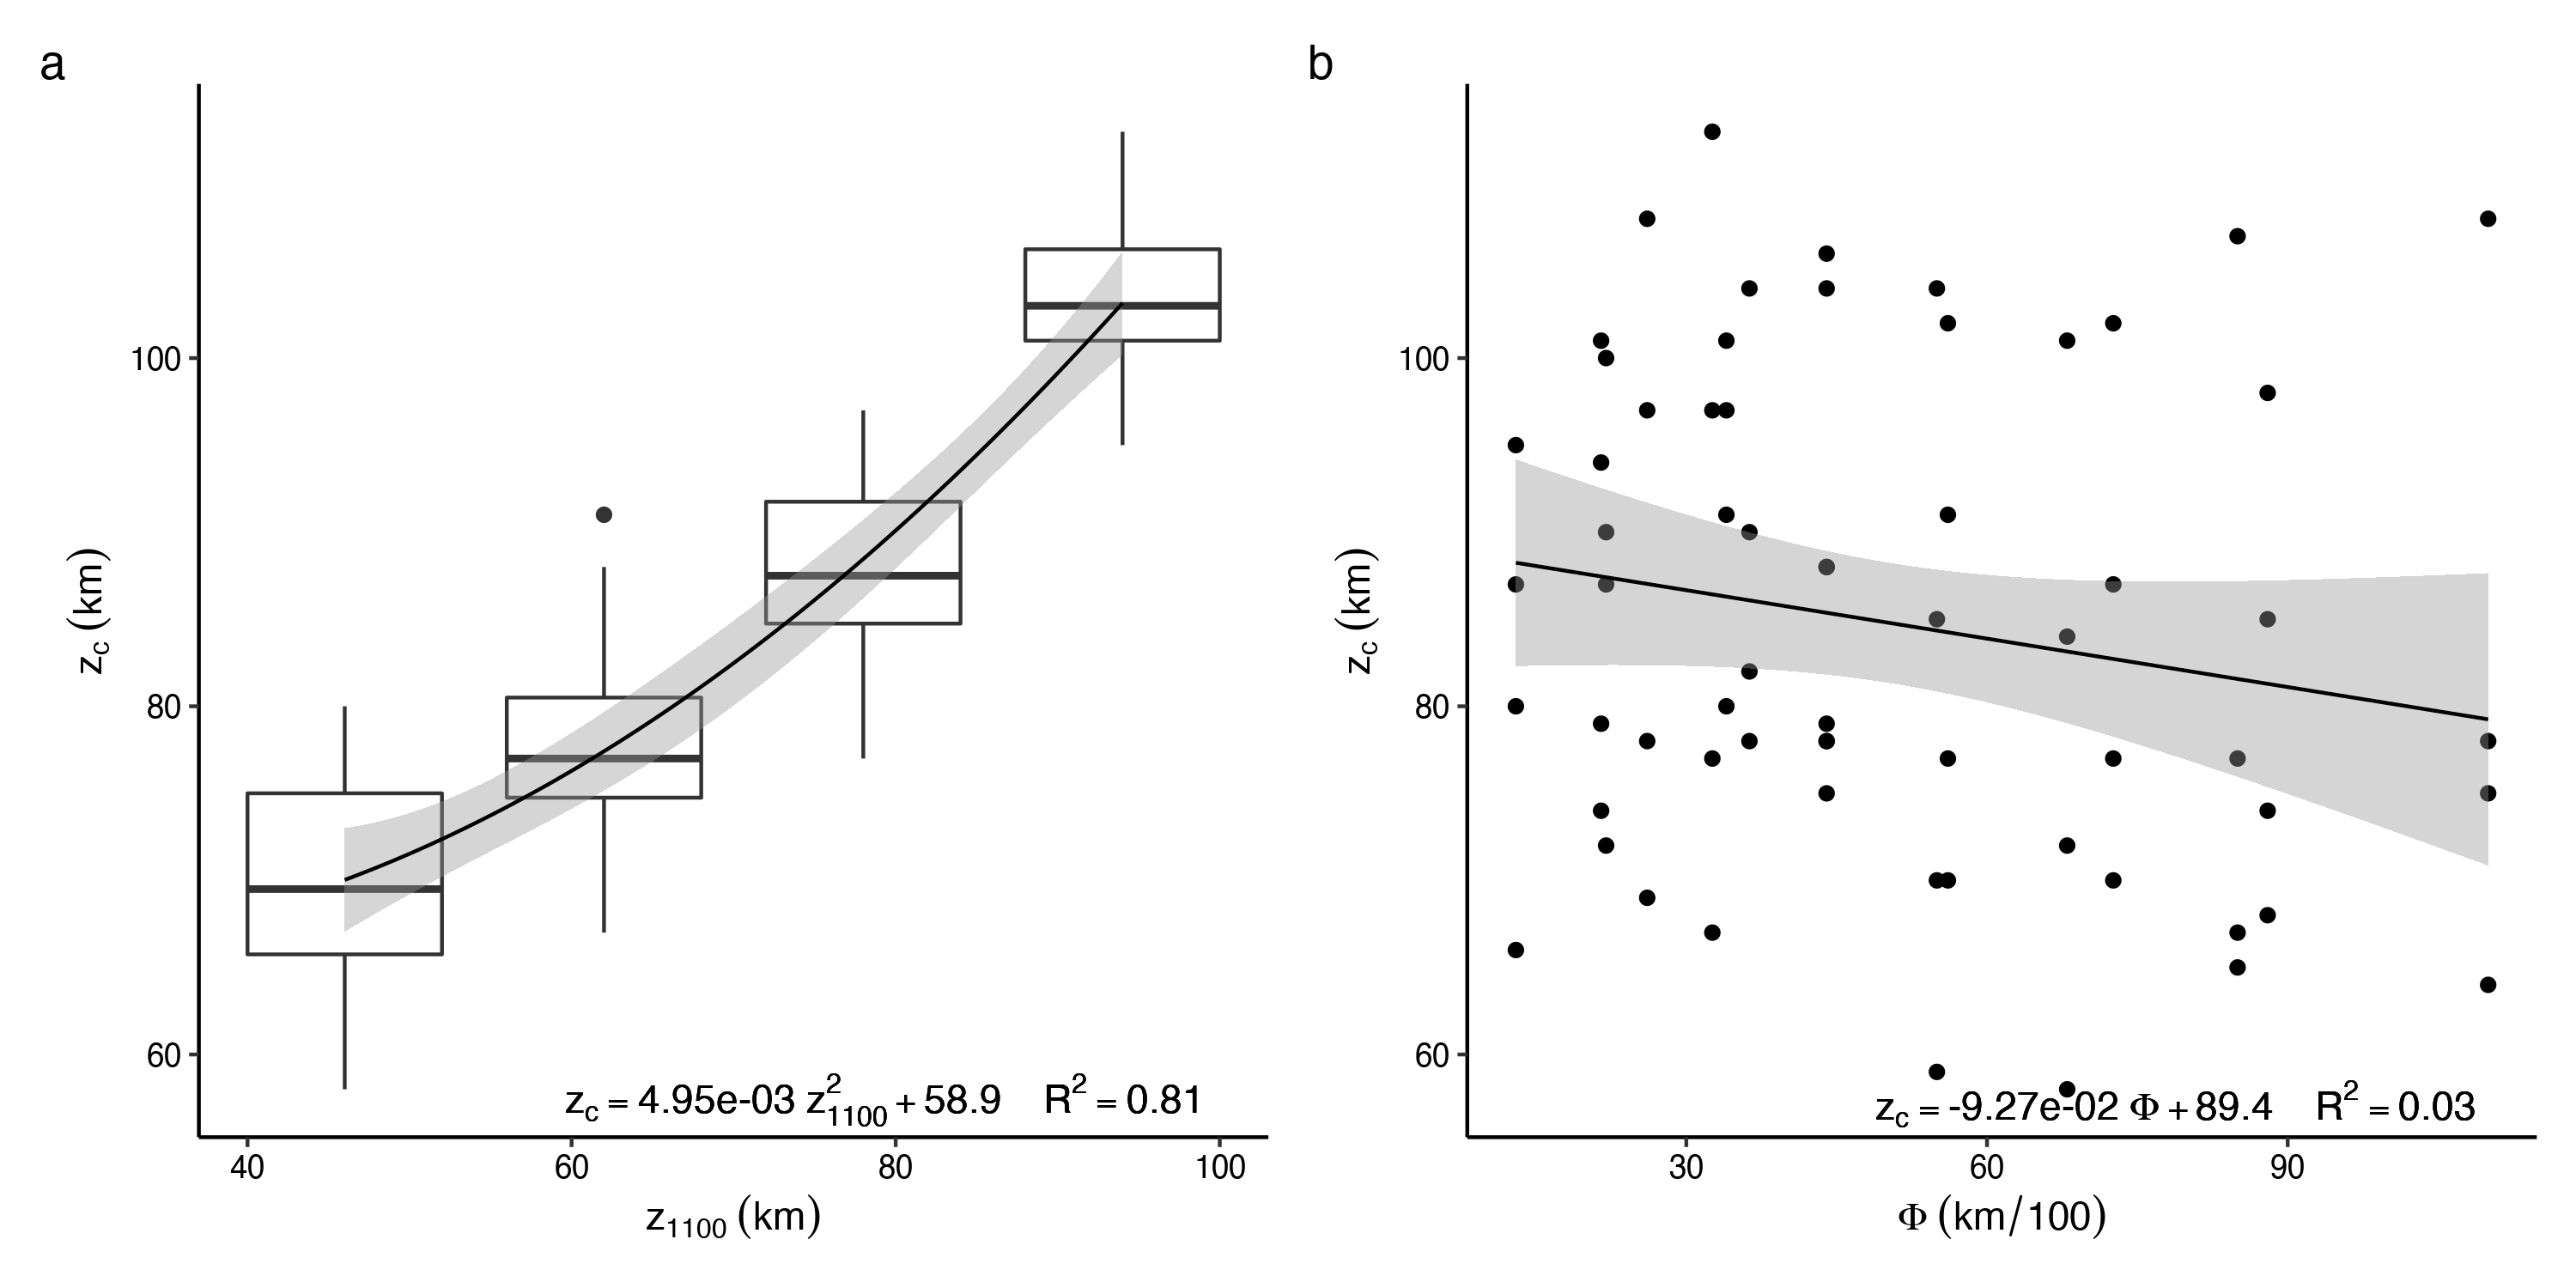
\includegraphics[width=\textwidth, trim={0 0 0 0}]{figs/Fig5.png}
 \caption{Single parameter regressions. (a) Coupling depth vs. thermal parameter. No significant correlation occurs between coupling depth and the slab thermal parameter (the slope is not significantly different than zero). The thermal state of the slab has little effect on coupling depth and cannot be used as a standalone predictor. (b) Coupling depth vs. lithospheric thickness. Coupling depth increases nonlinearly with increasing backarc lithospheric thickness and is best fit by a cubic curve. The correlation is highly significant (see Tables S1 and S2) and explains more than 80\% of the variance in coupling depth. Lithospheric thickness alone predicts coupling depth well.}
 \label{Figure5}
\end{figure}

In a plot of lithospheric thickness vs. slab thermal parameter (Fig.~\ref{Figure6}a), contours of coupling depth are shallowly sloped, indicating that lithospheric thickness is more important than slab thermal parameter in predicting coupling depth. The misfit between equation~\ref{Equation6} and model estimates is normally distributed, indicating an uncertainty in predicted coupling depth of 0 $\pm$ 11 $km$ (2$\sigma$; Fig.~\ref{Figure6}c). Predicted coupling depth for 17 modern subduction segments where backarc heat flow data are adequate for inverting for lithospheric thickness \cite<Fig.~\ref{Figure6}b; Table~\ref{Table4}; data from>[]{Wada2009} show a wide range of predicted coupling depths, similar to our model simulations. Predicted coupling depths for modern subduction zones are distributed normally, with a mean of $\sim$82 $km$ and variation of $\pm$ 14 $km$ (2$\sigma$; Fig.~\ref{Figure6}d).

\begin{threeparttable}
 \caption{Modern subduction zone segments}
 \label{Table4}
 \begin{tabularx}{\textwidth}{L{2} R{0.5} R{0.5} R{0.5} R{0.5} R{0.5}}

  \toprule

  Segment          & $z_{1100}$ & $\phi/100^1$ & $z_c$ & $q_s$    & References$^2$ \\

                   & $km$       & $km/100$     & $km$  & $mW/m^2$                  \\

  \midrule

  N. Cascadia      & 74.2       & 3.44         & 90.5  & 75       & 1              \\
  Nankai           & 96.3       & 6.9          & 109   & 69       & 1              \\
  Mexico           & 98.1       & 7.15         & 111   & 72       & 1
  \\
  Columbia-Ecuador & 66.4       & 10.4         & 84.5  & 80       & 2              \\
  S.C. Chile       & 66.4       & 20           & 83.6  & 80       & 2
  \\
  Kyushu           & 83.2       & 13.5         & 96.6  & 69       & 1
  \\
  N. Sumatra       & 26.8       & 25           & 64.8  & 120      & 3
  \\
  Alaska           & 66.4       & 25.3         & 83.1  & 80       & 2
  \\
  N. Chile         & 58.7       & 38.4         & 77.1  & 85       & 1
  \\
  N. Costa Rica    & 58.5       & 20.4         & 78.7  & 80       & 2
  \\
  Aleutians        & 51.6       & 39.6         & 73.1  & 75       & 1
  \\
  N. Hikurangi     & 58.5       & 41           & 76.7  & 80       & 2
  \\
  Mariana          & 47.5       & 54.6         & 69.7  & 80       & 2
  \\
  Kermadec         & 47.5       & 60           & 69.2  & 80       & 2
  \\
  Kamchatka        & 80.2       & 77           & 88.3  & 70       & 1
  \\
  Izu              & 47.5       & 77           & 67.6  & 80       & 2
  \\
  NE Japan         & 47.7       & 108          & 64.9  & 88       & 1
  \\

  \bottomrule
 \end{tabularx}
 \begin{tablenotes}
  \footnotesize
  \item [] $z_{1100}$=lithospheric thickness, $\phi$=thermal parameter, $z_c$=coupling depth, $q_s$=average backarc heatflow
  \item [1] $\phi = age \cdot convergence~velocity$; applicable to equation (5).
  \item [2] 1=\citeA{Currie2006} 2=\citeA{Currie2006} 3=\citeA{Wada2009}
 \end{tablenotes}
\end{threeparttable}

\begin{figure}
 \centering
 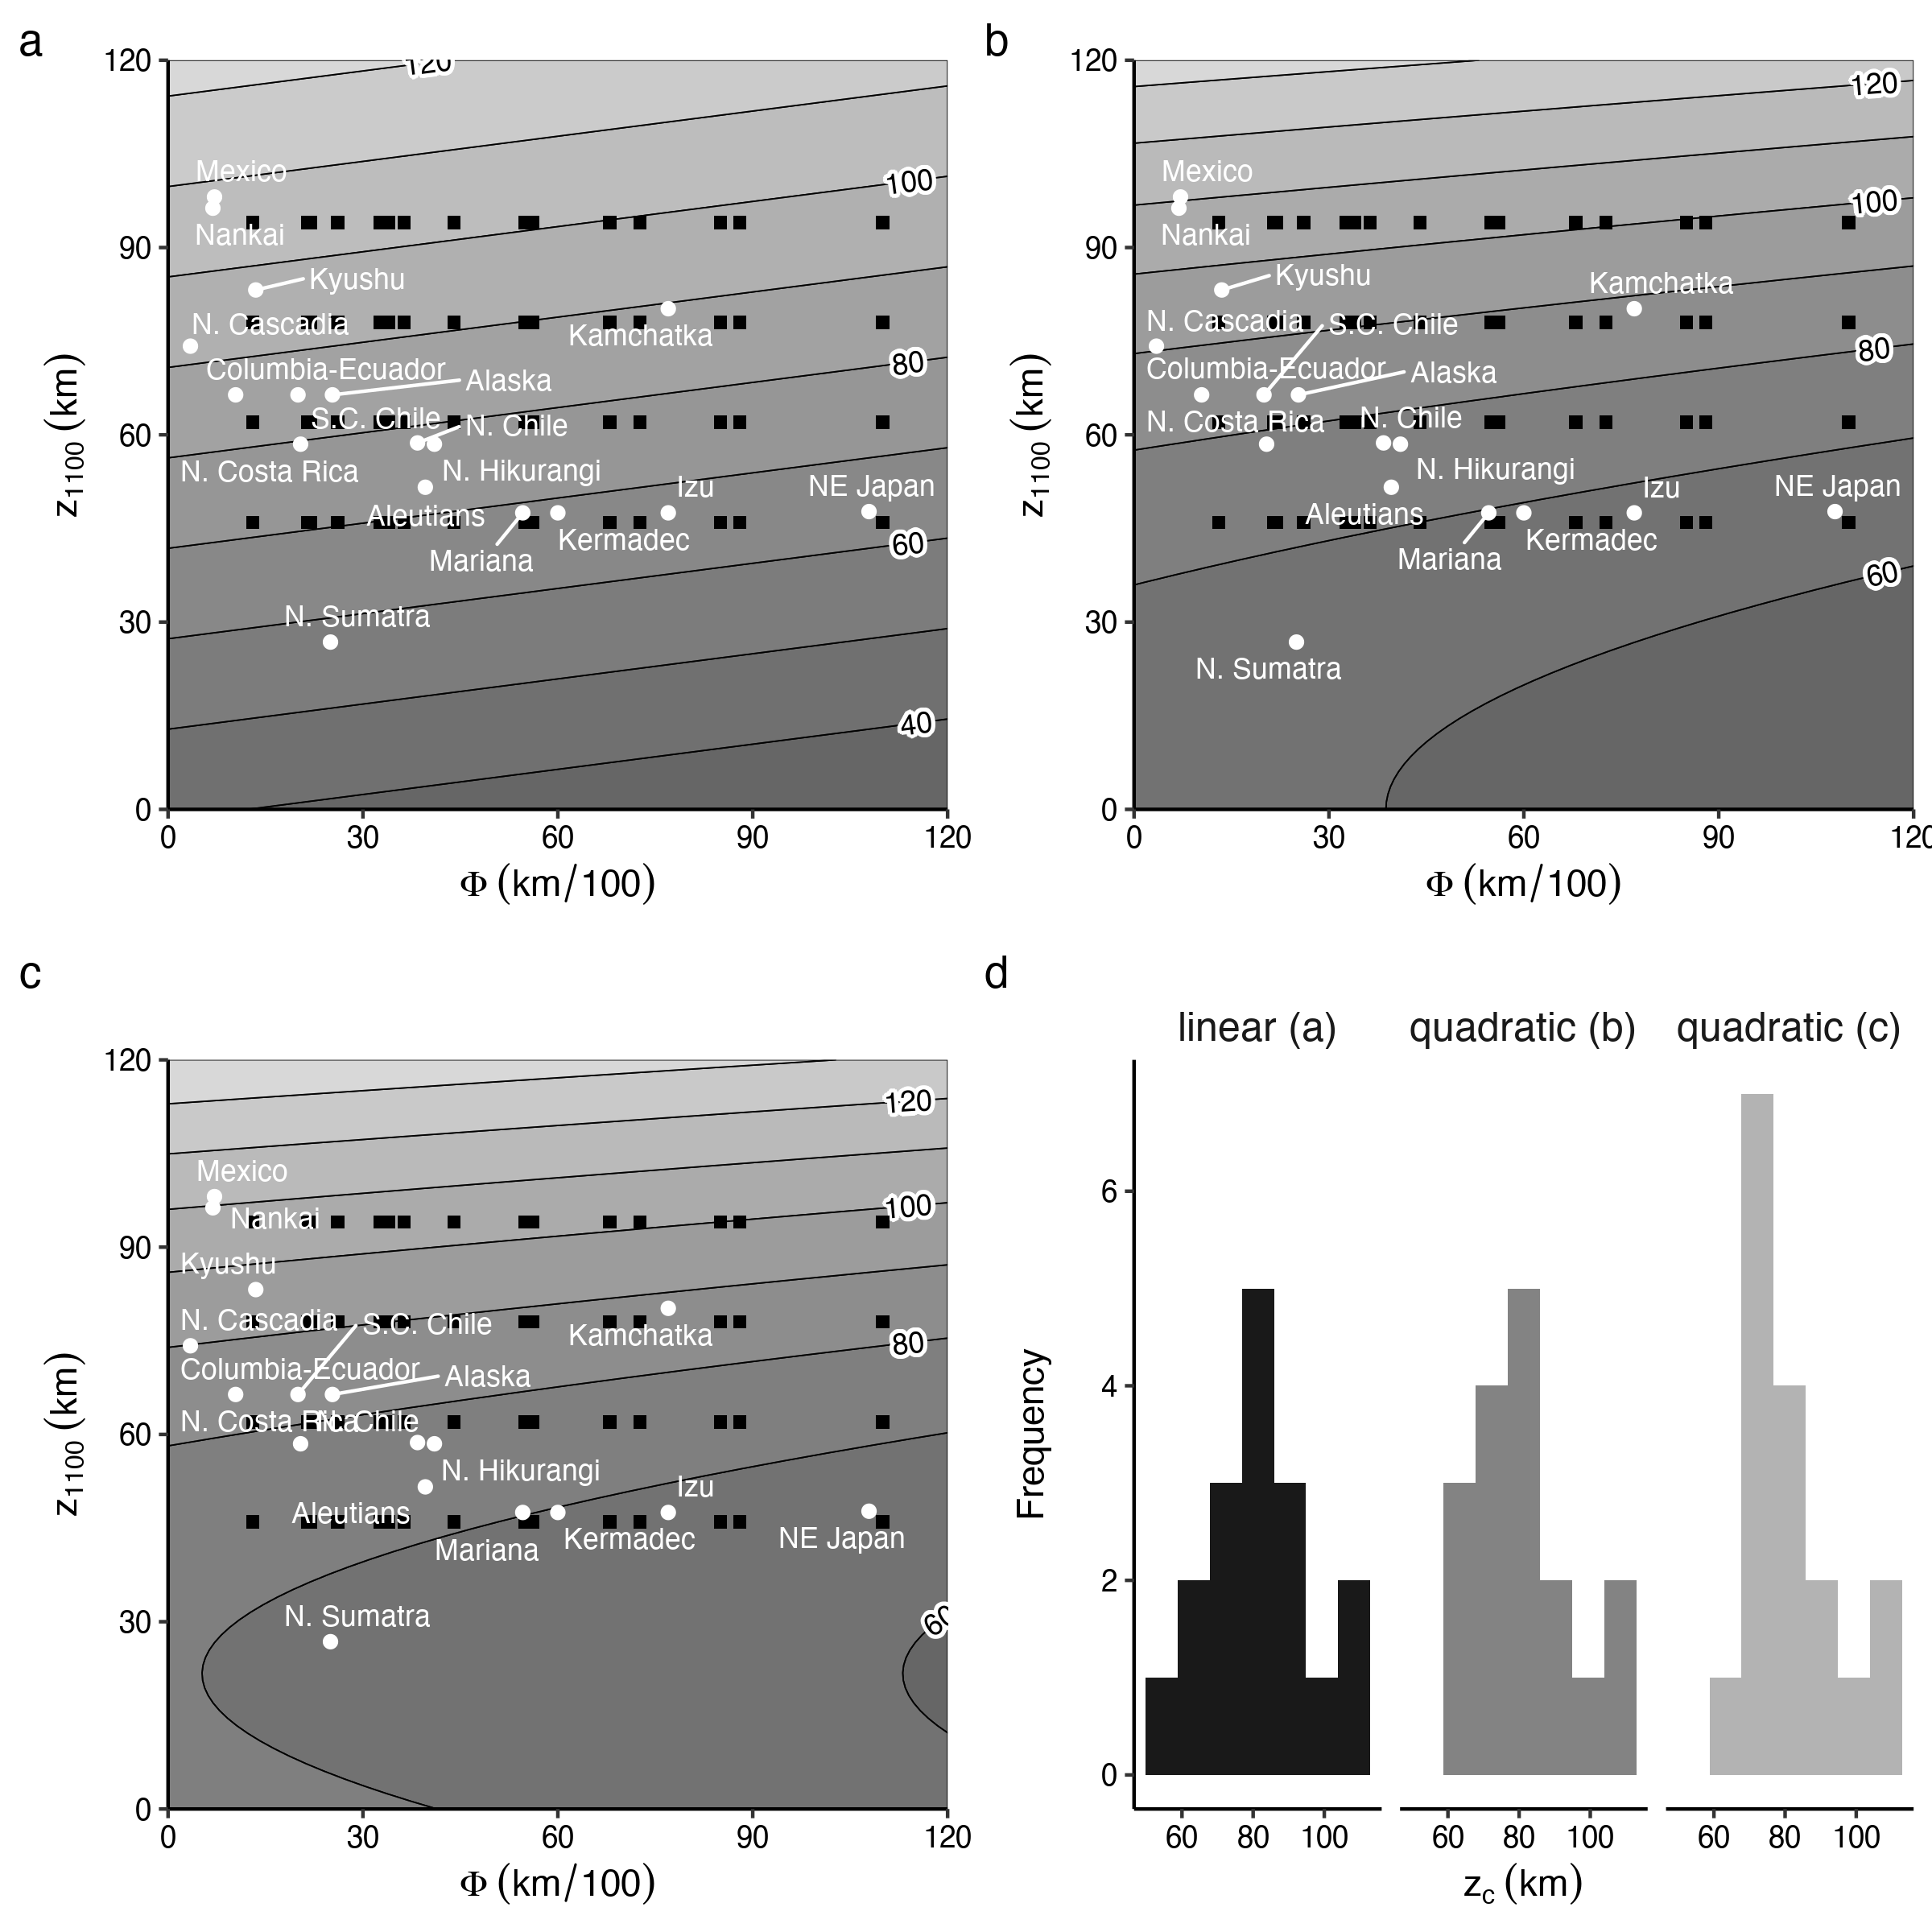
\includegraphics[width=\textwidth, trim={0 0 0 0}]{figs/Fig6.png}
 \caption{Multivariate regression and evaluation of predicted coupling depths for models and for present-day arc segments. (a) Contour plot shows predicted coupling depths (contours) as a function of slab thermal parameter and lithospheric thickness using our equation~\ref{Equation6}. Each data point represents one numerical model. The size and shades of the data points correspond to their measured coupling depth. Including thermal parameter improves quality of fit (see Table~\ref{TableS2}) although coupling depth depends much more strongly on lithospheric thickness than thermal parameter. (b) Plotting positions of 17 modern subduction zone segments based on data from \protect\cite{Wada2009}. Subduction systems with similar thermal parameters can have quite different predicted coupling depths (e.g., Alaska vs. N. Sumatra), while subduction systems with quite different thermal parameters can have quite similar predicted coupling depths (e.g., Kamchatka vs. N. Cascadia) (c) The difference between measured vs. predicted coupling depths for all 64 numerical models, indicating a precision of 0 $\pm$ 11 $km$. (d) Distribution of predicted coupling depths for the 17 modern subduction zones shown in (b). The light dashed line is the probability density of the data if Nankai and Mexico are considered outliers and excluded. Considering outliers does not significantly change the mean or median. These 17 segments span a large range of thermal parameters but are predicted to have coupling depths of 82 $\pm$ 14 $km$.}
 \label{Figure6}
\end{figure}

\subsection{Surface heat flow}
Calculated surface heat flow for numerical models with low to moderate slab thermal parameters (solid and short-dashed lines; Fig.~\ref{Figure7}) converge on uniform values of surface heat flow in the backarc region. However, all numerical models show some high-amplitude and high-frequency positive deviations in heat flow within the arc and backarc regions (Fig.~\ref{Figure7}), especially for the oldest slabs with the highest convergence rates (highest $\Phi$). These deviations correspond to strong extensional deformation and heat transport via lithospheric thinning and melt migration (long-dashed lines, Fig.~\ref{Figure7}). These heat flow excursions underscore the importance of characterizing extensional deformation and local advective heat transport by fluids before attempting to invert backarc lithospheric thickness from surface heat flow.

\begin{figure}
 \centering
 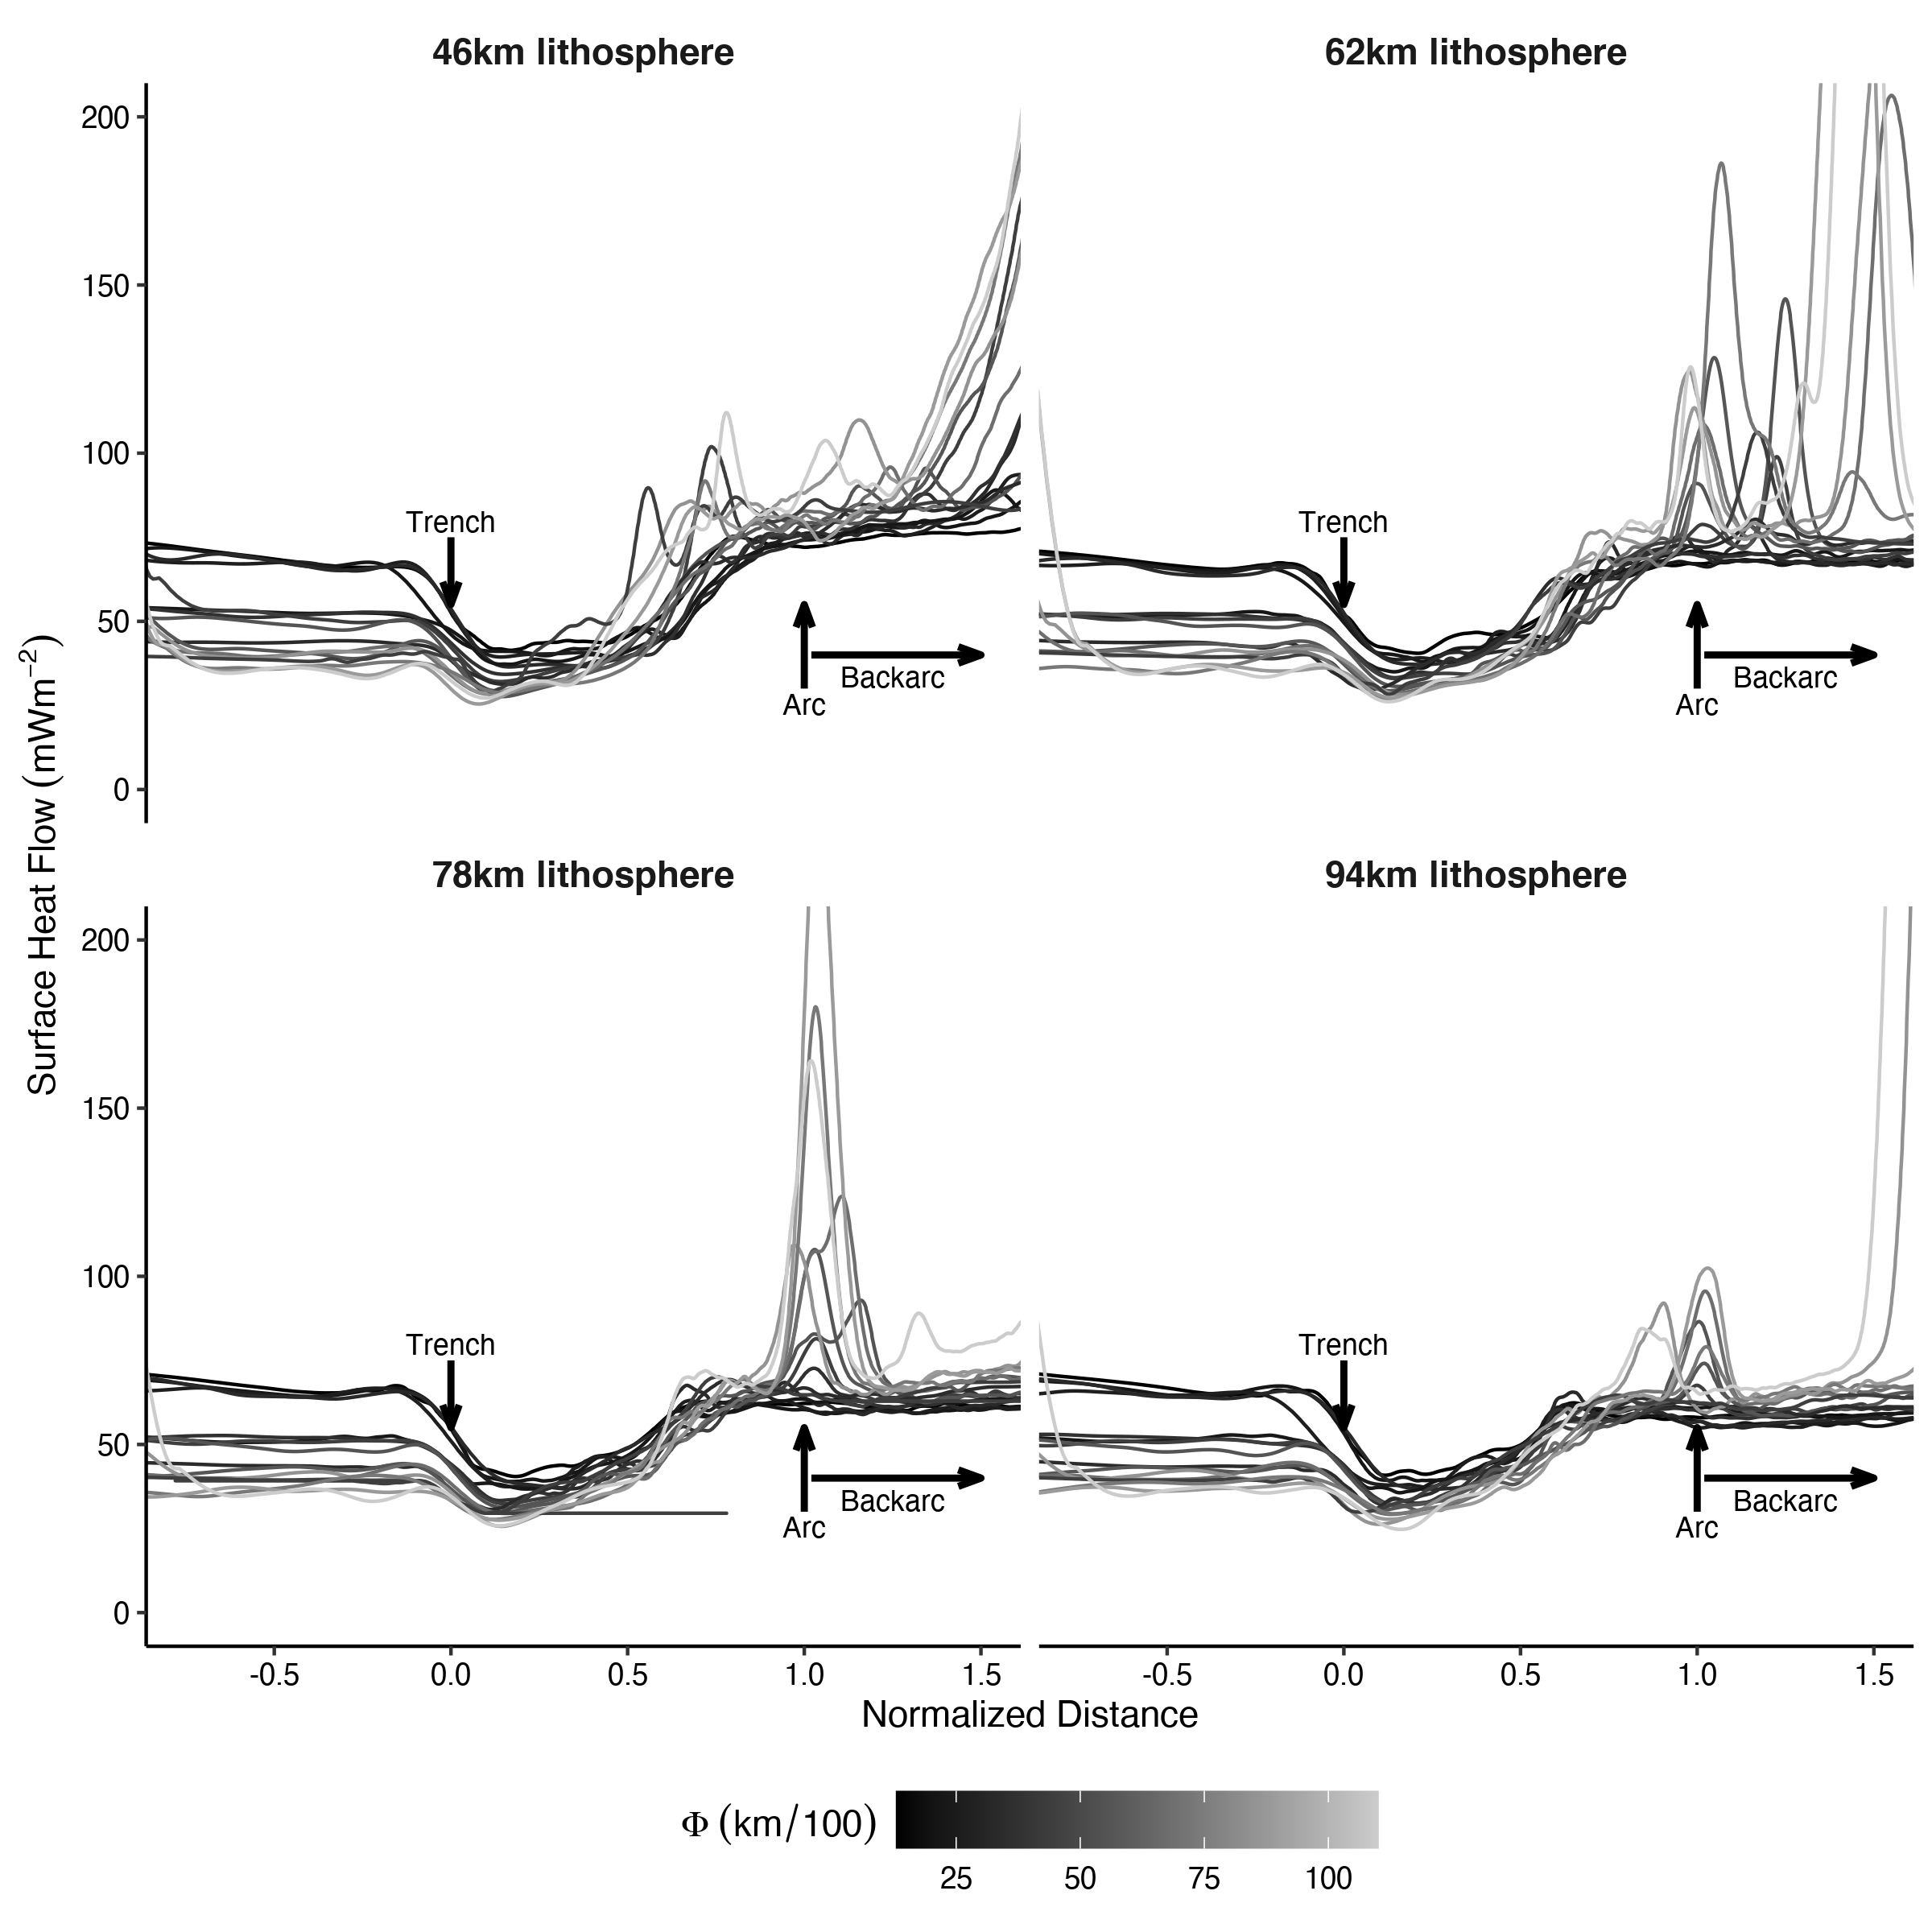
\includegraphics[width=\textwidth, trim={0 0 0 0}]{figs/Fig7.png}
 \caption{Surface heat flow calculations vs. normalized distance for models with backarc lithospheric thicknesses of (a) 46, (b) 62, (c) 78, and (d) 94 $km$. Normalized distance is the true distance relative to the trench divided by the distance between the arc and trench. Light grey lines show the entire range of heat flow values and bold lines emphasize models with low (cda), intermediate (cdf), and high (cdp) slab thermal parameters. High amplitude fluctuations in heat flow in the arc region (normalized distance $\approx$1.0) correspond to vertical migration of fluids and melts. In the backarc region, these fluctuations correspond to backarc extension associated with the oldest and fastest-moving slabs. Models with no extension fall within a narrow range of surface heat flow values in the backarc region.}
 \label{Figure7}
\end{figure}

A comparison of surface heat flow across numerical models with identical slabs, but varying backarc lithospheric thickness (model cdf with 46, 62, 78, and 94 $km$-thick lithospheres) shows very similar values of heat flow in the forearc (normalized distance $\leq$ 0.75; Fig.~\ref{Figure8}). In contrast, surface heat flow in the near-arc to backarc (normalized distance $>$ 0.75; Fig.~\ref{Figure8}) disperses systematically and reflects initial steady-state continental geotherms (i.e. lithospheric thickness).

\begin{figure}
 \centering
 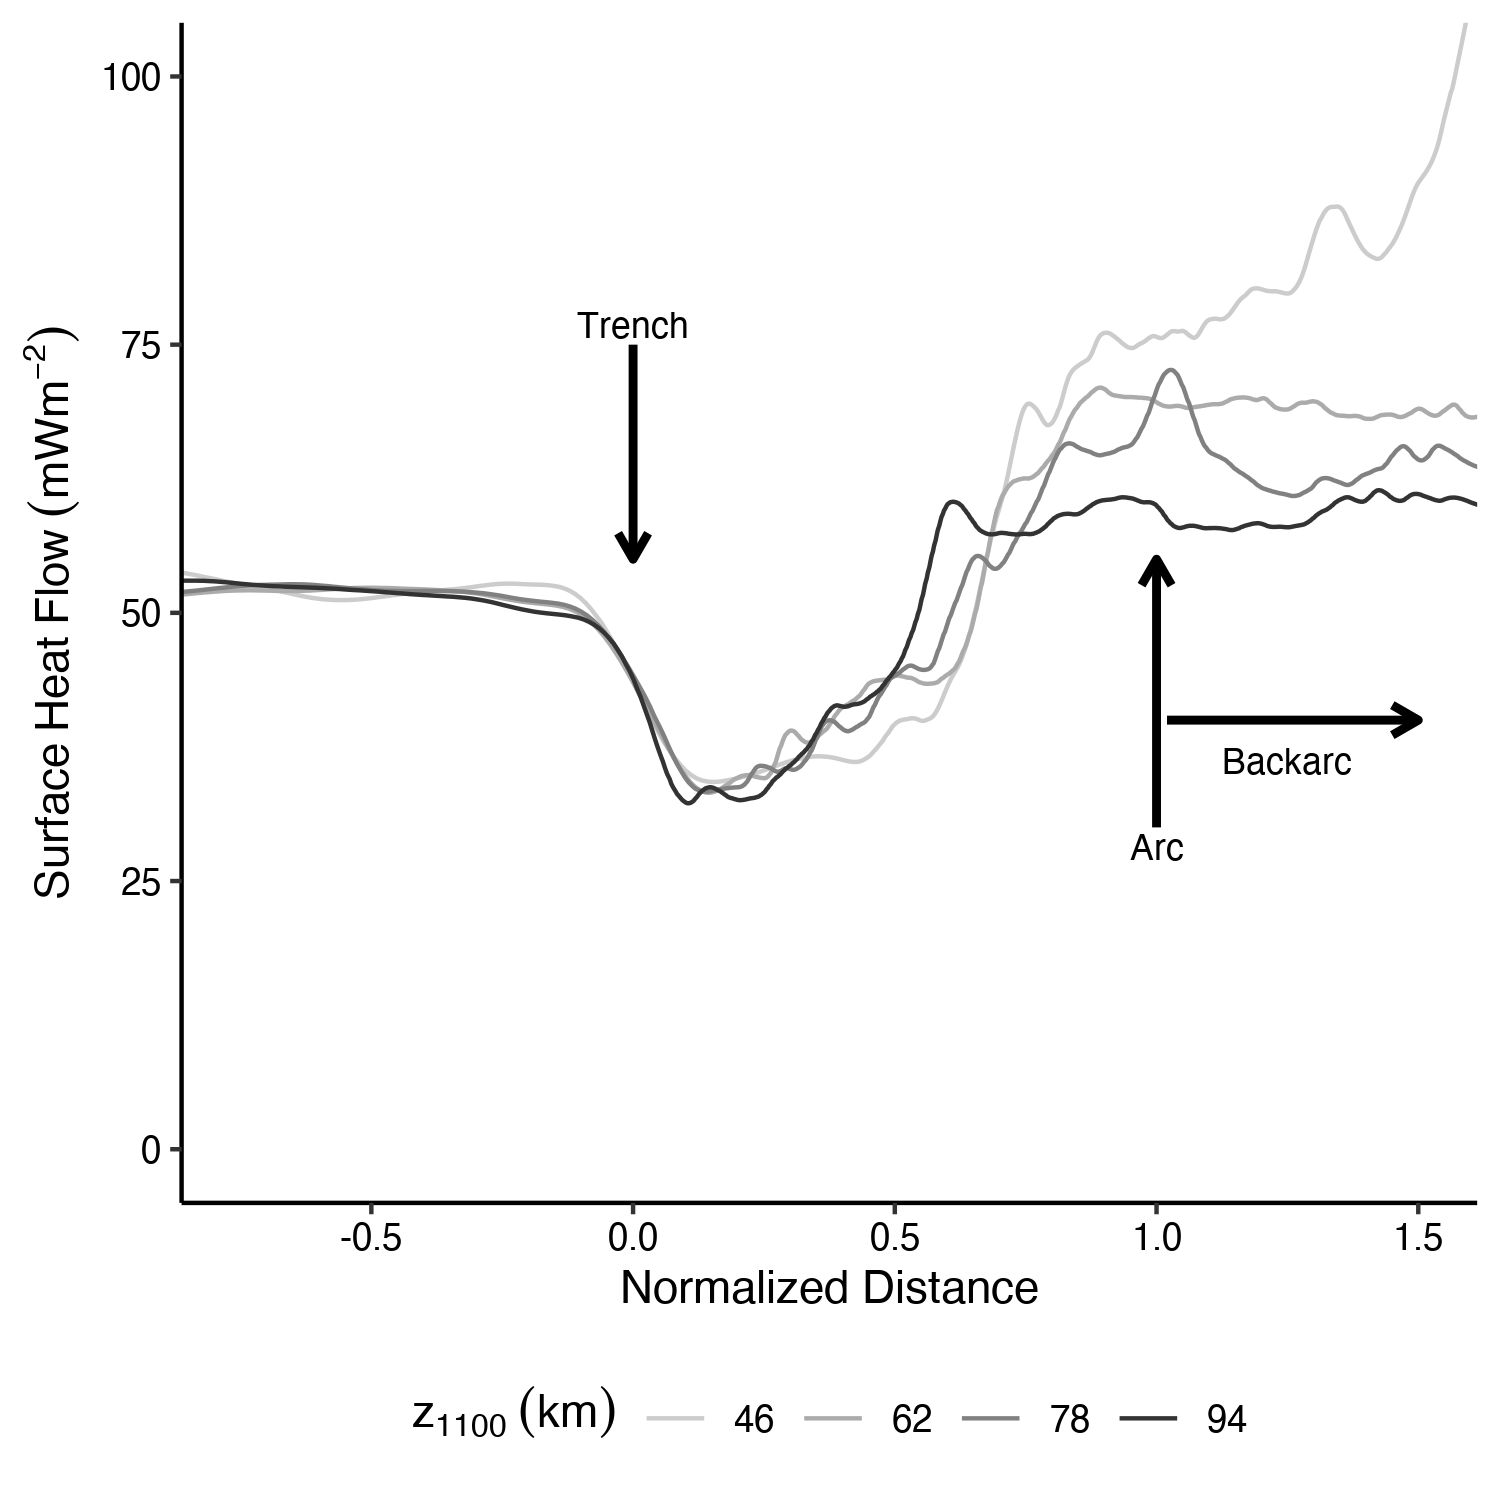
\includegraphics[width=0.5\textwidth, trim={0 0 0 0}]{figs/Fig8.png}
 \caption{Surface heat flow vs. normalized distance for model cdf with backarc lithospheric thicknesses ranging from 46 to 94 $km$. The range of surface heat flow values in the forearc (normalized distance between 0.0 and 1.0) is narrow and shows little dispersion until near the arc (normalized distance between 0.75 and 1.0). Surface heat flow broadly disperses in the backarc (normalized distance $>$ 1.0) and reflects the initial continental geotherm (lithospheric thickness). A simple relationship between surface heat flow and lithospheric thickness may be obscured in any region experiencing an addition of heat from extension or vertical migration of fluids, especially within the arc-region.}
 \label{Figure8}
\end{figure}

\section{Discussion}
\subsection{Reaction Mechanism and Thermal Controls on Slab-Mantle Mechanical coupling}
In our numerical experiments, slab-mantle mechanical coupling is spatially associated with the reaction of (weak) antigorite to form (stronger) wet olivine. An antigorite-rich serpentinized subduction channel spontaneously forms atop the dehydrating slab, localizing strain, lubricating the slab-mantle interface, and mechanically decoupling the slab and mantle wedge \cite<e.g.,>[]{Ruh2015, Agard2016}. As anticipated, it is the viscosity increase resulting from the transformation of antigorite ($\eta \approx 10^17$) to wet olivine ($\eta \approx 10^23$) that causes slab-mantle mechanical coupling in our models, where the depth of this reaction is primarily controlled by a balance of competing thermal feedbacks acting in the upper plate. Cooling and hydration of the upper lithospheric mantle wedge (antigorite stabilization) and heating from the lower circulating asthenospheric mantle wedge (antigorite destabilization) compete to fix the antigorite-out reaction at depth (Fig.~\ref{Figure9}).

\begin{figure}
 \centering
 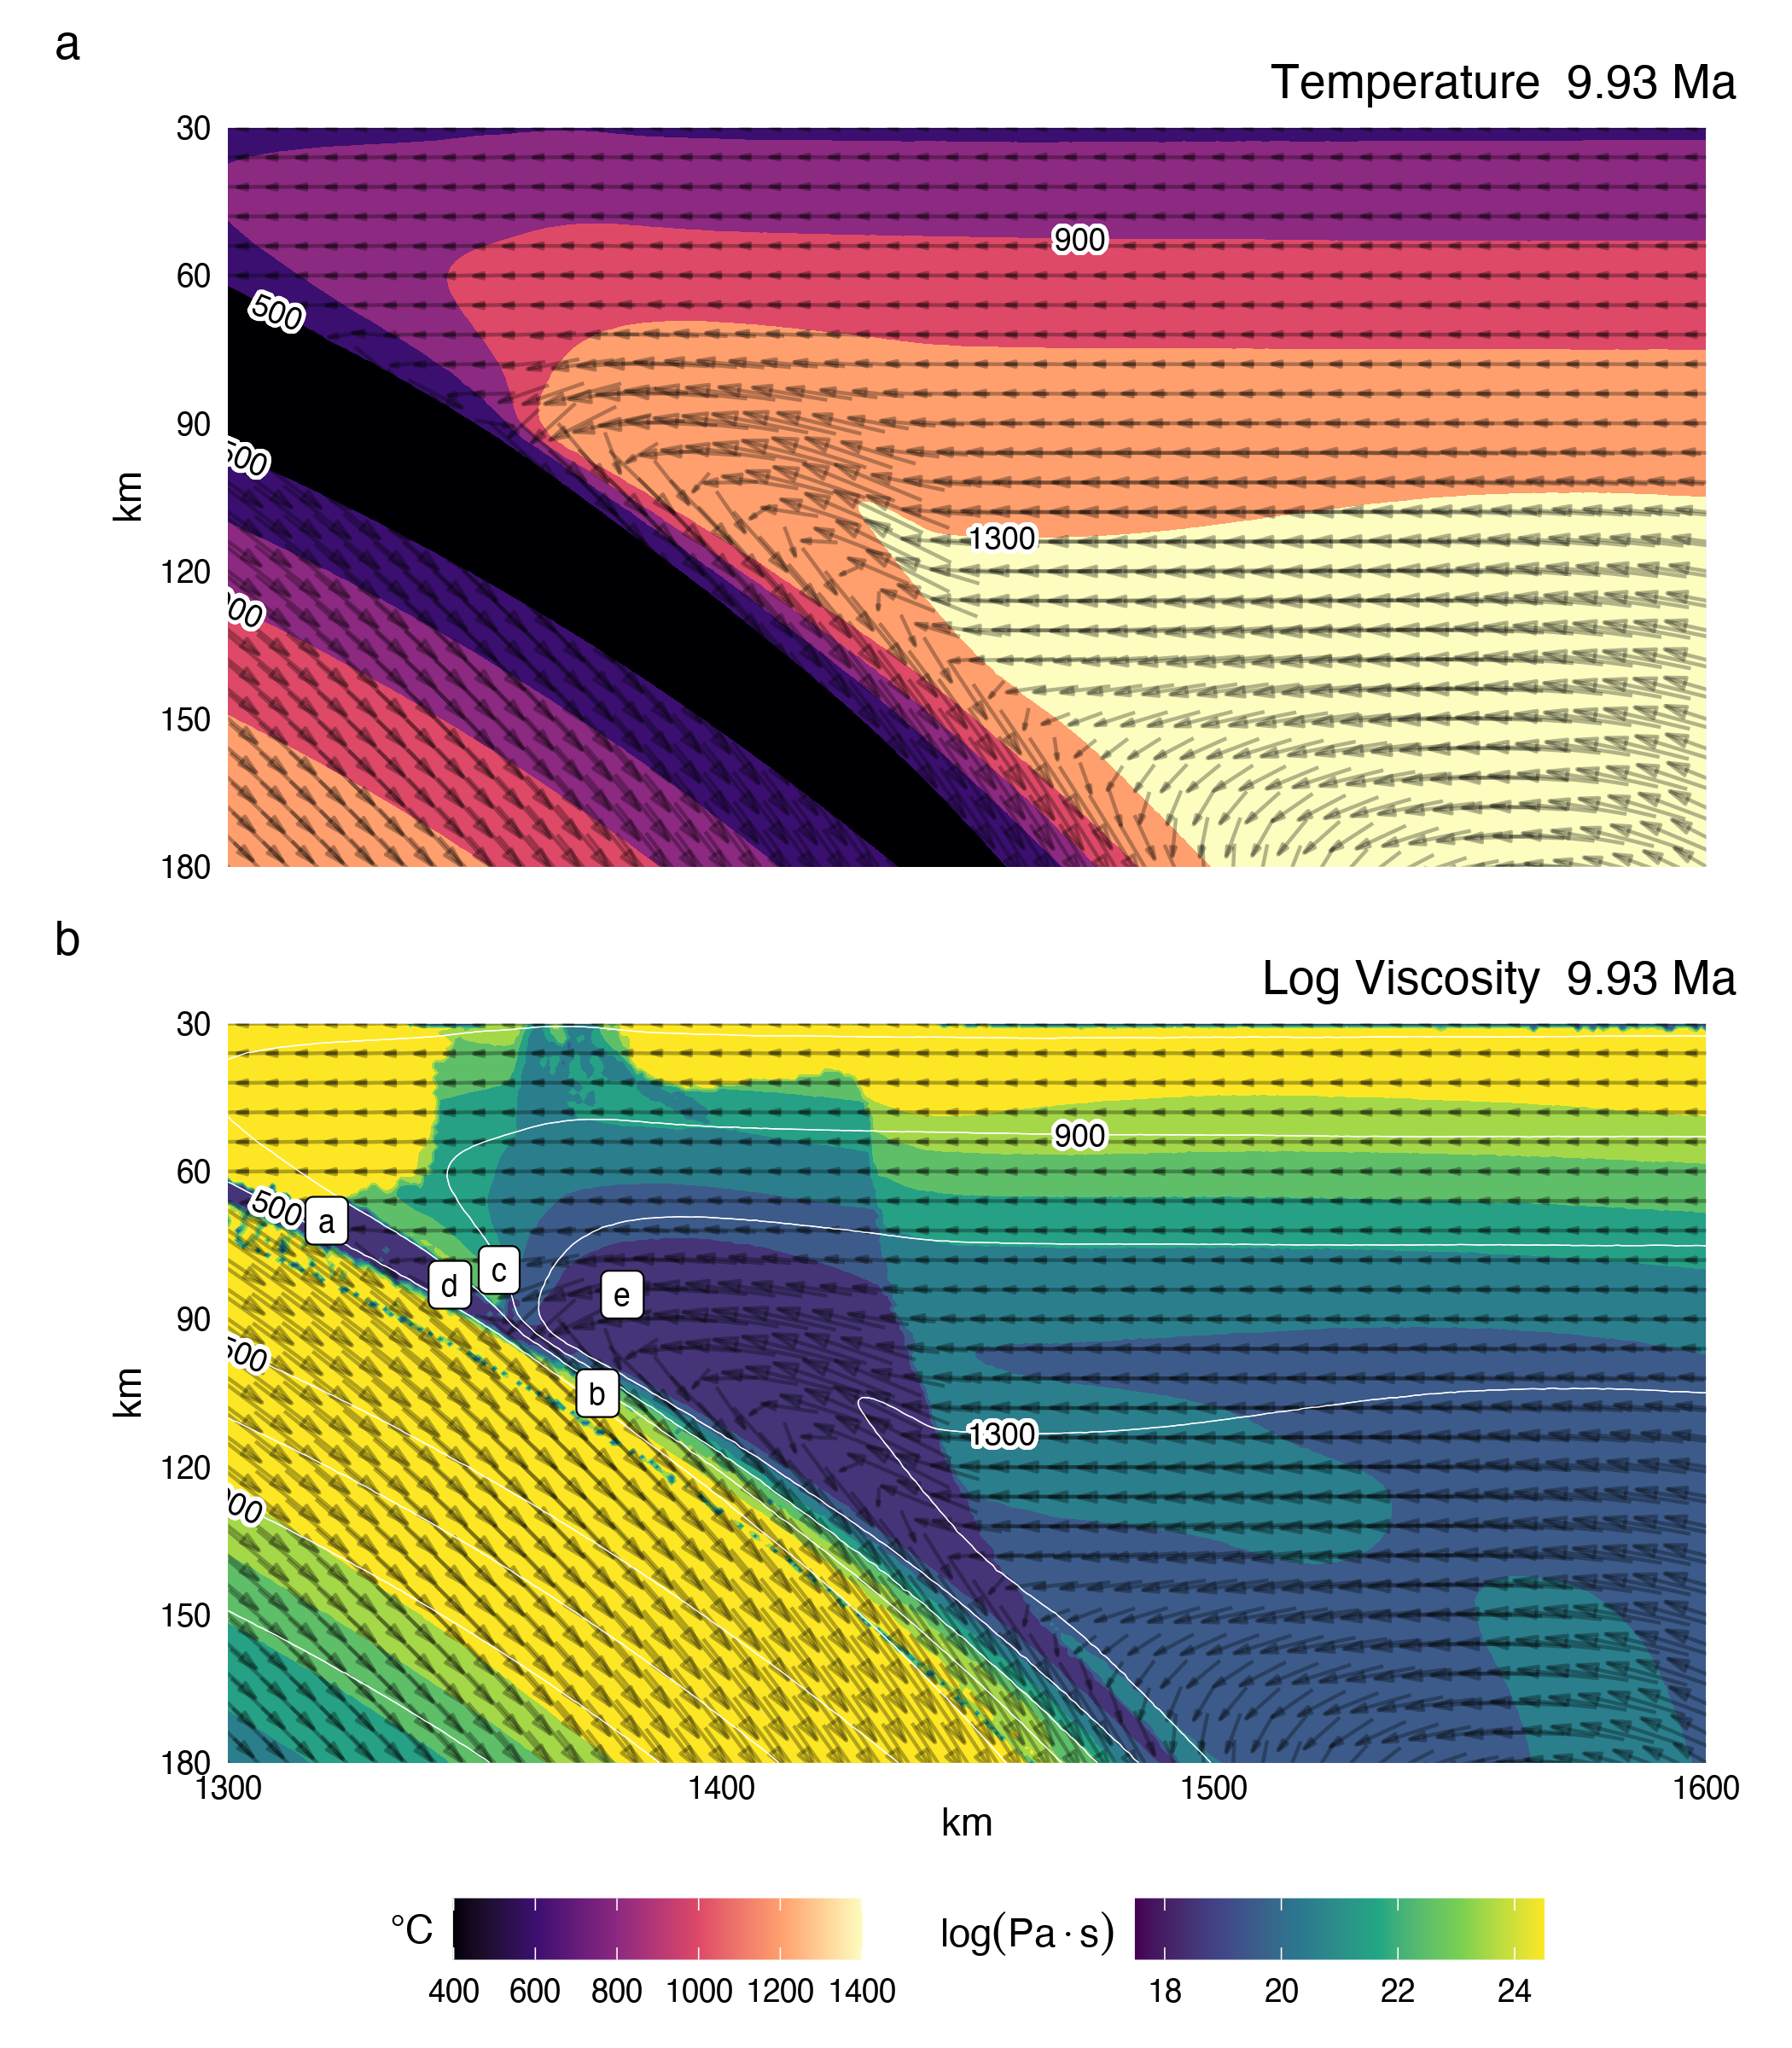
\includegraphics[width=\textwidth, trim={0 0 0 0}]{figs/Fig9.png}
 \caption{Visualization of an effective P\'{e}clet number and viscosity near the coupling region at $\sim$10 $Ma$ for model cdf with lithospheric thickness of 78 $km$. (a) Effective P\'{e}clet number. Advection dominates transport of heat towards the coupling point (thin dark red region in the asthenospheric mantle wedge), whereas diffusion contributes significantly to transport of heat away from the coupling point by the slab (yellow-green region within the slab). (b) Viscosity. Coupling occurs at the point where the viscosity contrast between the slab and mantle approaches zero. The layer of small cyan-green dots of lower viscosity in the slab reflect serpentine alteration that occurred along bending faults near the trench. Reference points a-e are used for discussing reaction mechanisms and thermal feedbacks during the transition to slab-mantle mechanical coupling.}
 \label{Figure9}
\end{figure}

The entire process can be conceptualized in terms of an effective P\'{e}clet number. Cooling of the mantle wedge occurs mainly via diffusive heat loss to the slab along the entire length of the subducted slab-top, as indicated by the bowed isotherms and relatively low (-20 $<$ Pe $<$ 20) effective P\'{e}clet values along the slab-mantle interface (Fig.~\ref{Figure9}a). At shallow levels, water released from the slab stabilizes serpentine in the overriding mantle, effectively decoupling the slab mechanically from the mantle (Fig.~\ref{Figure9}b, point a). This mechanical decoupling promotes antigorite stabilization to greater depths because the mantle wedge stagnates and continues to cool and receive water from the dehydrating slab\textemdash a positive feedback for the formation of serpentinite. Stagnation is evident by near-zero effective P\'{e}clet values within the lithospheric mantle wedge (Fig.~\ref{Figure9}a). We note that the warm-colored band that tracks the minimum thermal gradient does not indicate unusually efficient advective heat transport (the numerator of equation~\ref{Equation5} is not especially large), but rather inefficient diffusive heat transport in the context of a small thermal gradient (the denominator of equation~\ref{Equation5} is small).

At deeper levels, beyond the stability of antigorite, diffusive heat loss from the mantle to the slab forms a thickening layer of new lithosphere atop the slab (Fig.~\ref{Figure9}b, point b). Downward motion of this new lithosphere (Fig.~\ref{Figure9}b, point b) relative to the deepest extent of the stiff forearc mantle (Fig.~\ref{Figure9}b, point c) creates a pressure gradient that attracts flow of the weakest materials\textemdash serpentinite from the up-dip direction (Fig.~\ref{Figure9}, point d)\textemdash and hot mantle from below (Fig.~\ref{Figure9}, point e). Flow of hot mantle into the necking region between points b and c is analogous to passive asthenospheric upwelling toward a mid-ocean ridge where two strong cooling lithospheric plates diverge. Highly efficient heat advection from the warm mantle wedge core (dark red stream at T $>$ 1100 $^{\circ}C$; Fig.~\ref{Figure9}a) drives reaction of serpentinite to form wet olivine\textemdash a negative feedback to the formation of serpentinite.

It is the finely-tuned balance of serpentine stability\textemdash the addition of water into a diffusively cooling, shallow mantle to produce serpentine vs. the advection of heat from the deeper mantle to prevent it\textemdash that defines the coupling depth.

\subsection{The impact of $z_{1100}$ and $\Phi$ on coupling}
How does backarc lithospheric thickness ($z_{1100}$) influence coupling depth? The lithosphere\allowbreak-asthenosphere boundary of the upper plate defines the permissible flow field of circulating upper mantle, limiting highly efficient heat advection to below the base of the mechanical lithosphere (c.f. Fig.~\ref{Figure10}a-d). Thin upper plate lithospheres (Fig.~\ref{Figure10}a, b) permit shallower mantle wedge circulation and advection of heat farther up the subduction interface. This shallow circulation raises the depth of the serpentine breakdown reaction and mechanical coupling. Thick upper plate lithospheres (Fig.~\ref{Figure10}c, d) restrict mantle wedge circulation and advection of heat to deeper levels, shifting the serpentine breakdown reaction and mechanical coupling to greater depths.

\begin{figure}
 \centering
 \includegraphics[width=\textwidth,  trim={0 0 0 0}]{figs/Fig10.png}
 \caption{Variation in effective P\'{e}clet number for the standard model, cdf, with backarc lithospheric thickness of (a) 46, (b) 62, (c) 78, and (d) 94 $km$. All models are visualized at $\sim$10 $Ma$ and plotted on the same scale and location within the model domain. All models display broadly similar distributions of an effective P\'{e}clet number, but the thin dark red streams focus on the subduction interface at different depths. In each model, the thin red stream flowing towards the coupling point is limited to the base of the upper-plate lithosphere, $z_{1100}$.}
 \label{Figure10}
\end{figure}

In our models, the thermal state of the slab, as represented by the thermal parameter ($\Phi$), has almost no effect on the mechanical coupling depth. Previous studies of modern subduction zones also concluded that coupling appears to be insensitive to slab age and convergence velocity \cite{Furukawa1993, Wada2009}. The likely reason that $\Phi$ makes so little difference is because slab dynamics drive mantle wedge circulation and mantle wedge cooling in opposite directions. High-$\Phi$ slabs (older slabs with higher velocities) cool the mantle wedge more effectively, but also result in stronger mantle circulation and greater heat advection. In contrast, low-$\Phi$ slabs (younger slabs with lower velocities) are less effective in cooling the mantle wedge, but also result in weaker mantle circulation and less heat advection. That is, the shallow vs. deep impacts of $\Phi$ tend to cancel each other, explaining the lack of strong correlation between coupling and thermal parameter.

\subsection{Predicting Coupling Depths in Subduction Zones}
Theoretically, coupling depth can be predicted directly from forearc heat flow using forward modelling techniques to fit surface heat flow data \cite<e.g.,>[]{Wada2009}. However, we caution against using fore-arc heat flow data because a) forward models adjust the mechanical coupling depth independently from the backarc thermal structure, which is inconsistent with the inherent link between mechanical coupling and backarc thermal structure discussed above (e.g., Figs.~\ref{Figure8},~\ref{Figure10}), b) data are typically sparser in the forearc region compared to the backarc region  \cite{Currie2006}, and c) shear heating and crustal plutonism can contribute to surface heat flow in the forearc \cite{Gao2014, ReesJones2018}, complicating any simple correspondence with coupling depth.

Instead, we recommend predicting mechanical coupling depth in modern subduction zones based on equation~\ref{Equation6} and estimates of backarc lithospheric thickness (as estimated from backarc heat flow) and slab thermal parameter. The slab thermal parameter is inventoried for most subduction zone segments \cite{Syracuse2006}, but a corresponding dataset of lithospheric thicknesses does not exist. Several geophysical and petrologic methods might be considered for independent estimates of lithospheric thickness (e.g., seismic velocities, flexure, heat flow, mantle xenoliths, etc.), but we prefer to focus on backarc surface heat flow because of its direct correspondence with thermal structure. In this approach, backarc lithospheric thickness is estimated using simple one-dimensional heat transport models assuming values for radiogenic heat production in the crust \cite<e.g.,>[]{Rudnick1998}. That is, one can use compiled backarc heat flow data to invert for backarc lithospheric thickness, calculate the slab thermal parameter from the product of slab age and convergence velocity, and apply equation~\ref{Equation6} to estimate mechanical coupling depth. Of course, care must be taken to avoid backarcs with strong extensional deformation or conspicuous heating from magmatism because heat flow in these regions will underestimate backarc lithospheric thickness and consequently underestimate coupling depth.

\subsection{A Common Coupling Depth Globally?}
Mechanical coupling depths in subduction zones are commonly assumed to fall within a narrow range of 70-80 $km$ \cite{Wada2009, Syracuse2010}.  We tested the correlation between backarc lithospheric thickness and coupling depth using the natural dataset compiled by \citeA{Wada2009} (Fig.~\ref{Figure6}b, d). Much of their dataset is based on \citeA{Currie2006}, who infer backarc lithospheric thicknesses for 10 circum-Pacific subduction zones of 50-60 $km$ (as defined by the 1200 $^{\circ}C$ isotherm). Backarc lithospheres are inferred to be relatively thin from uniformly high heat flow ($>$ 70 $mW/m^2$), thermobarometric constraints on mantle xenoliths, and P-wave velocities \cite{Currie2006}. The mean value of 82 $\pm$ 14 $km$ (2$\sigma$) for mechanical coupling depths in our analysis (Fig.~\ref{Figure6}d) roughly matches the preferred depth inferred from forearc heat flow data for Cascadia and NE Japan \cite<75-80 $km$;>[]{Wada2009, Syracuse2010}, but our predicted coupling depths (Fig.~\ref{Figure6}d) are distributed more broadly. For example, omitting Mexico and Nankai because their $\Phi$ values fall outside our modeling domain, predicted coupling depths range from $\sim$100 $km$ (Kyushu) to $\sim$65 $km$ (Sumatra and NE Japan).

The petrologic record may also provide insight into the consistency of a mechanical coupling depth. As it approaches the mechanical coupling depth, the serpentine channel narrows and focuses return flow. The demise of the serpentine channel at greater depths may provide a natural barrier such that rocks within the serpentine channel are more likely to be exhumed than rocks below the channel. If so, the abundance of blueschists and eclogites whose maximum burial depths are less than the pinchout of the serpentine channel, i.e., at the mechanical coupling depth, should be greater than rocks with greater maximum burial depths. A cumulative probability distribution of data compiled by \citeA{Penniston2015} shows a distinct kink at an inferred depth of $\sim$80 $km$ (Fig.~\ref{FigureS2}). Rocks whose peak metamorphic pressures correspond with depths $\leq$ 80 $km$ are much more likely to be exhumed than rocks metamorphosed at depths $>$ 80 $km$. In fact, nearly all examples of rocks exhumed from greater depths in the compilation of \citeA{Penniston2015} were exhumed in the context of collisions. Logically, the metamorphic record supports a common mechanical coupling depth of $\leq$~80 $km$.

Relatively high backarc heat flow (especially in circum-Pacific subduction zones) suggests relatively stable and uniformly thin backarc lithospheres in mature subduction zones globally that may in turn cause a common depth of slab-mantle coupling. Although we do not yet fully understand why the overriding plates may have similar thicknesses, we can assume that this is likely related to some processes of lithospheric erosion proposed for subarc lithosphere \cite<e.g.,>[]{Sobolev2005, Arcay2006, England2010}. The following mechanisms of lithospheric erosion have been proposed: lithospheric delamination induced by lower crust eclogitization \cite<e.g.,>[]{Sobolev2005}, small-scale convection caused by hydration-induced mantle wedge weakening \cite<e.g.,>[]{Arcay2006}, thermal erosion \cite<e.g.,>[]{England2010} and mechanical weakening \cite<e.g.,>[]{Gerya2011} by percolating melts and subarc foundering of magmatic cumulates \cite<e.g.,>[]{Jull2001}. Most of these mechanisms are thus strongly related to mantle wedge hydration, melting, and melt transportation toward volcanic arcs.

\section{Conclusions}
Four important results are highlighted in this study:

\begin{enumerate}
 \item The antigorite to olivine dehydration reaction stabilizes where balance is achieved between competing thermal feedbacks within the stagnant mantle wedge lithosphere (diffusive heat loss and inefficient heat advection) and circulating mantle wedge asthenosphere (highly efficient and focused heat advection). The depth of this reaction, and thus mechanical coupling, is primarily dependent on the mechanical thickness of the backarc lithosphere.

 \item A simple expression fitted to the results of our numerical models allows the mechanical coupling depth to be calculated for subduction zone segments with adequate surface heat flow data in the backarc region. Back-arc lithospheric thickness can be inferred from surface heat flow using a one-dimensional steady-state conductive cooling model. Together with slab thermal parameter , which is tabulated for nearly all subduction segments worldwide \cite{Syracuse2006, Syracuse2010}, coupling depth can be calculated using equation~\ref{Equation6}.

 \item Consistently high backarc heat flow in circum-Pacific subduction zones \cite{Currie2006, Wada2009} may indicate a common depth of slab-mantle mechanical coupling globally at ca. 80 $km$. Prior assumptions of slab-mantle mechanical coupling at 70-80 $km$ in thermal models is consistent with our results..

 \item As others have proposed \cite{Currie2006, Wada2009} subduction zones appear to self-organize into stable configurations globally with warm (thin) upper plate lithospheres and slab-mantle mechanical coupling at depths of ca. 80 $km$. Questions remain, however, including: 1) How do warm (thin) backarcs persist over 100's of kilometers throughout the lifespan of subduction zones? 2) How abrupt is the antigorite-out reaction along the subduction interface?, and 3) How can predictive models like equation~\ref{Equation6} be improved using natural datasets? We propose these questions as topics for future research.

\end{enumerate}

\appendix
\section{}
\subsection*{Subduction duration to achieve steady state}
In our models, the stability depth of antigorite along the slab-mantle interface increases with time as the subducting slab cools and hydrates the mantle wedge. We observed this process proceeding for the first 5 $Ma$ of subduction with the antigorite stability depth remaining constant for ca. 10 $Ma$ afterwards (Fig.~\ref{FigureS1}). The change in the antigorite stability depth, and therefore the slab-mantle mechanical coupling depth, through ca. 10 $Ma$ emerges self-consistently in our models and can help explain how similar configurations, in terms of the depth to the slab beneath arcs \cite{England2004} and thin backarc lithospheres \cite{Currie2006}, occur in subduction zones with different slab ages, convergence rates, geometries, and subduction durations. Our modelling results indicate that subduction zones quickly ($<$ 5 $Ma$) develop and stabilize quasi-permanent, generalized configurations with a slab-mantle mechanical coupling depth dependent on the thickness of the backarc lithosphere.

Exceptions occur in our models with the thinnest backarc lithospheres ($z_{1100}$ = 46 $km$), which exhibited transient behavior after ca. 5 $Ma$ (Fig.~\ref{FigureS1}a). Our models rapidly ($<$ 5 $Ma$) develop spreading centers in the backarc for these models because of their extremely thin (weak) backarc lithospheres. The proximity of a spreading center in the backarc region could divert enough heat from the circulating mantle wedge to stabilize antigorite to deeper levels in the forearc than in a similar system that does not develop a backarc spreading center. This may be tested by artificially increasing the strength of the backarc lithosphere for models with very thin backarc lithospheres.

\subsection*{Absolute minimum coupling depths?}
The form of our preferred quadratic regression model shows shallowing of coupling depths decelerating with progressively thinner upper plate lithospheres, reaching a minimum of ca. 60 $km$. This implies that the antigorite-out reaction should eventually stabilize at $\geq$ 60 $km$ depth even during nascent subduction and in warm systems with thin upper plate lithospheres. From a theoretical point of view, a thin upper plate lithosphere could allow high heat transport to the shallow mantle wedge and hinder stabilization of antigorite all together. Olivine plus pyroxene would be the stable mantle minerals and strong, shallow coupling between plates would be expected \cite{Gerya2008}. However, our models show that even the warmest subduction systems eventually stabilize antigorite in the shallow mantle wedge. This is evident by the increasing depth of mechanical coupling with time for the first 5 $Ma$ of subduction (Fig.~\ref{FigureS1}).

\begin{figure}[H]
 \centering
 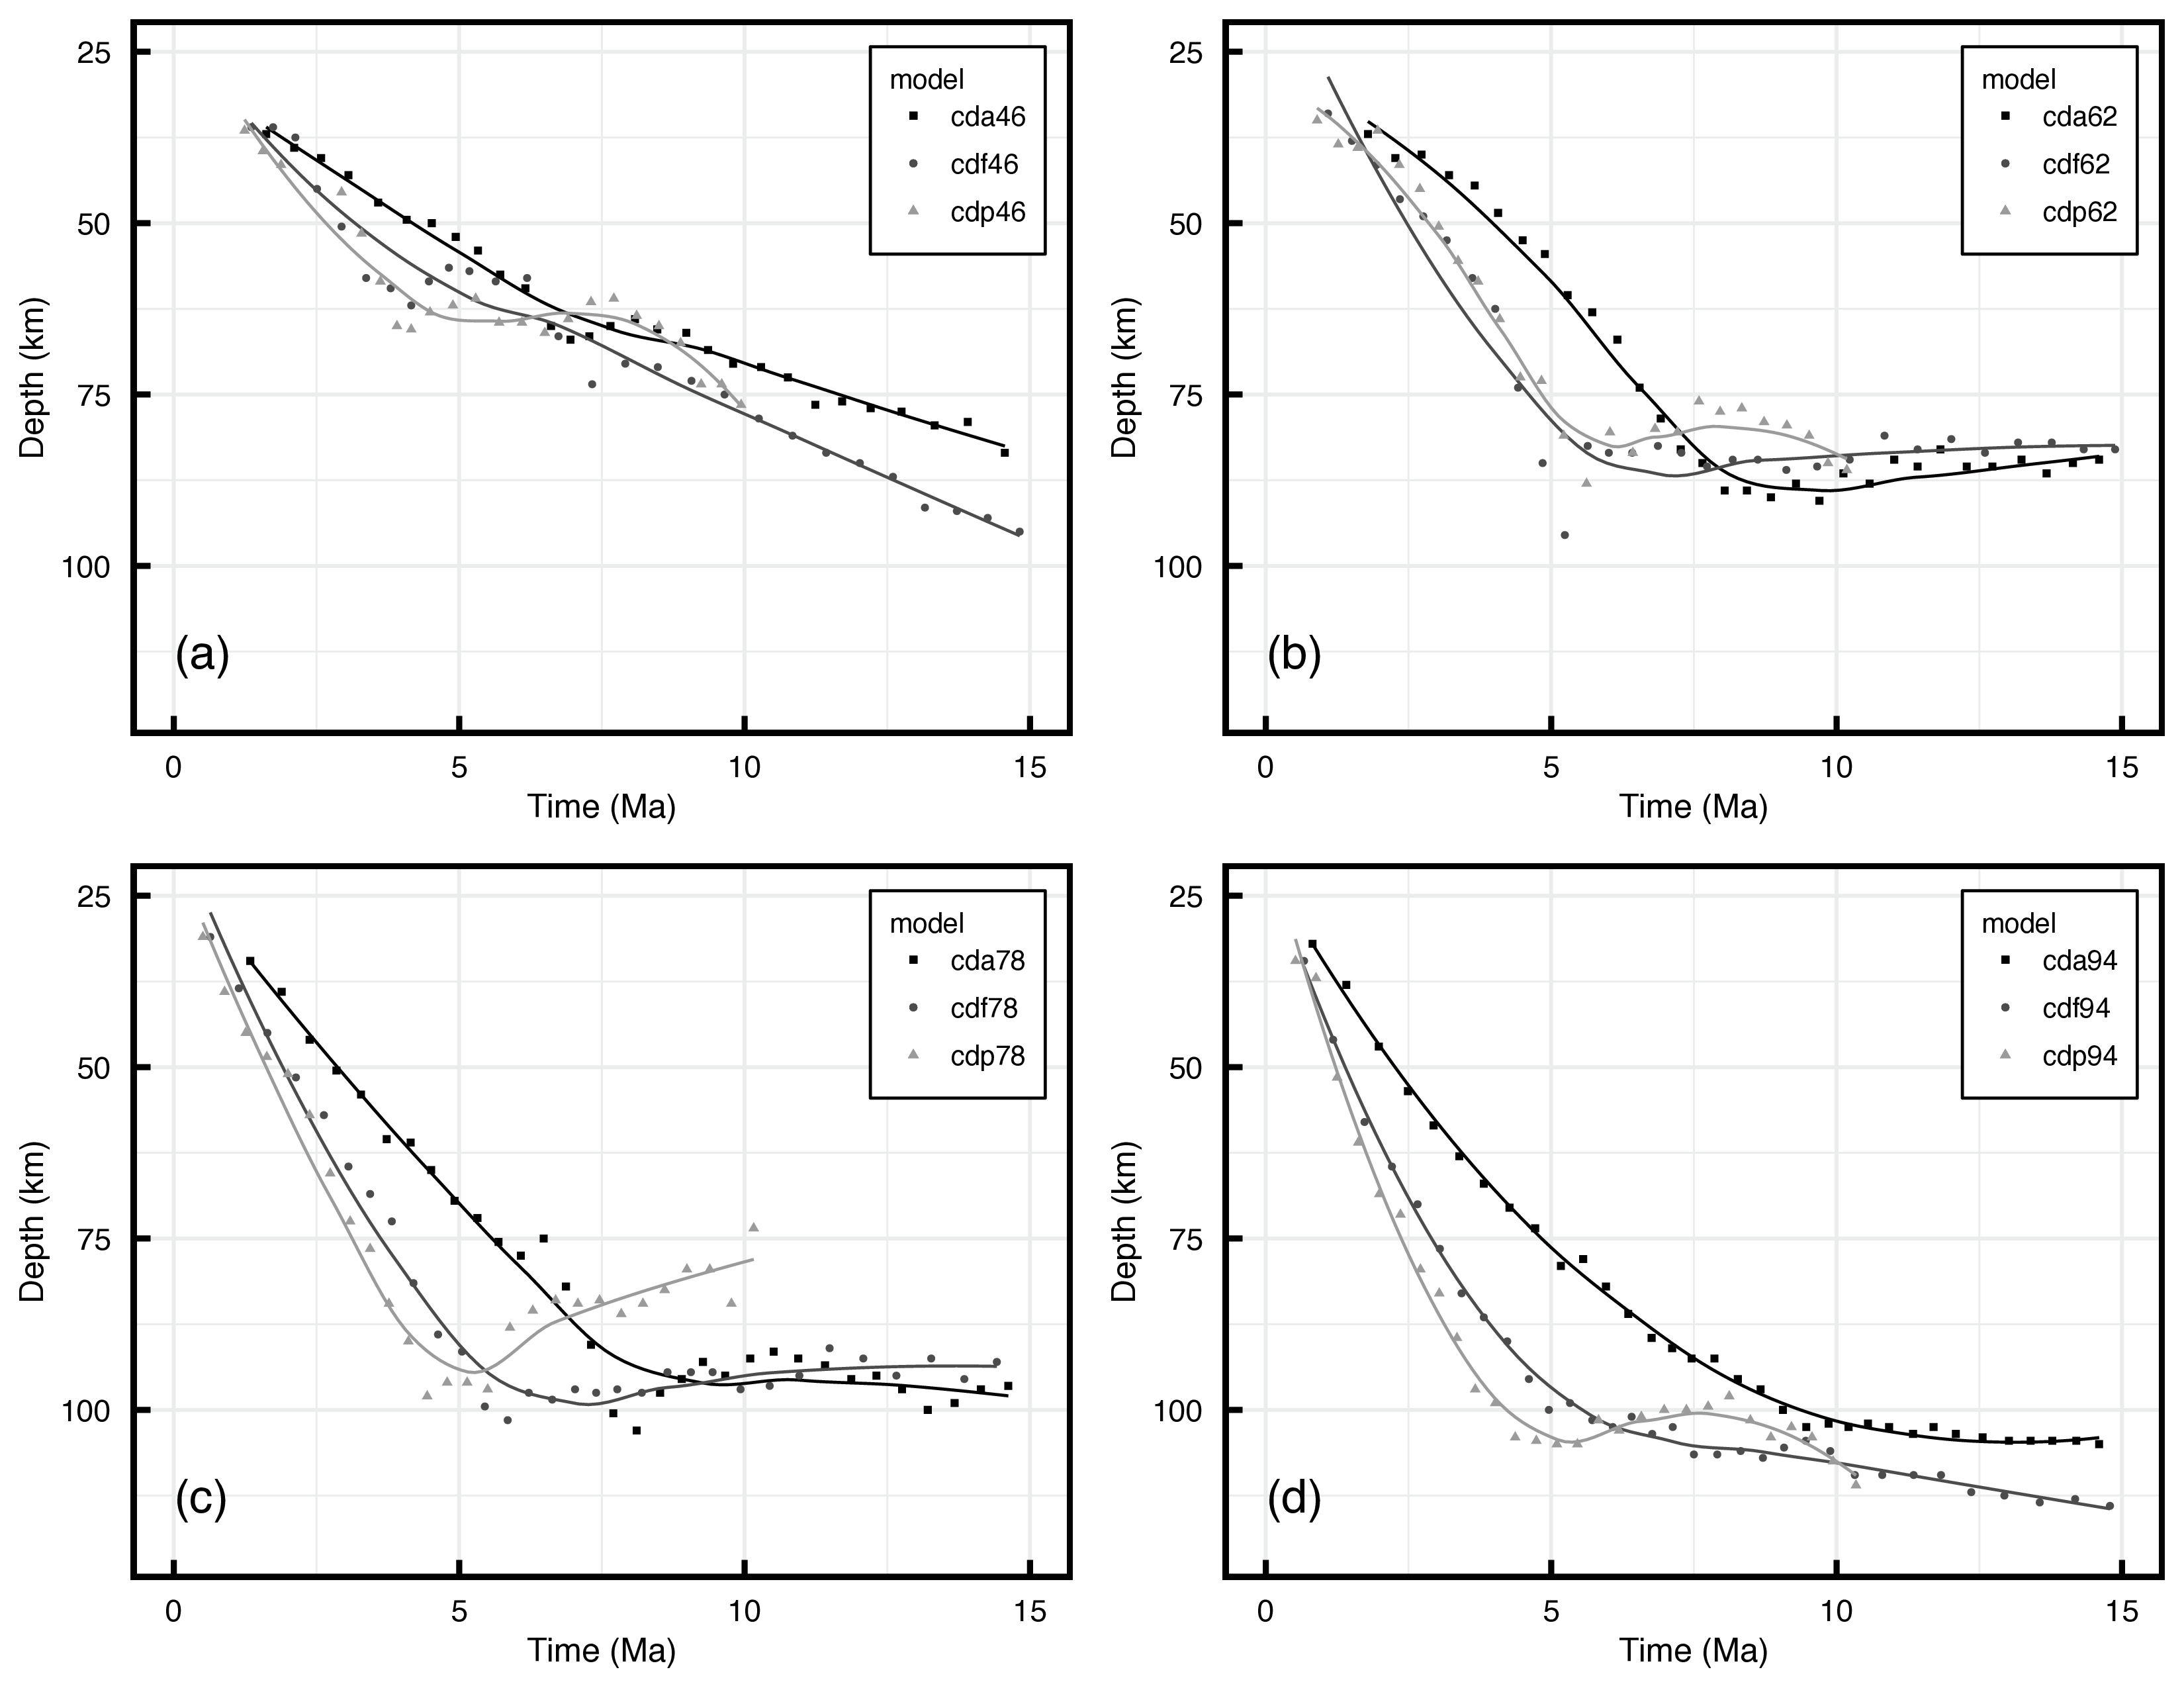
\includegraphics[width=\textwidth,  trim={0 0 0 0}]{figs/FigS1.png}
 \caption{The depth of antigorite stability at the slab-mantle interface vs. time for models with 46 (a), 62 (b), 78 (c), and 94 $km$-thick (d) backarc lithospheres. Antigorite stabilization deepens for the first ca. 5 $Ma$ of subduction and then remains roughly constant for ca. 10 $Ma$. The exceptions are models with very thin backarc lithospheres (a), which exhibit transient behavior for at least 15 $Ma$. The final achieved stability depth of antigorite increases with increasing backarc lithospheric thickness.}
 \label{FigureS1}
\end{figure}

\subsection*{(De-)hydration model}
The material properties used in our experiments are listed in Table~\ref{Table1} \& Table~\ref{Table2}. For details about the sedimentation and erosion, melting and extraction, and rheological models, please refer to \citeA{Sizova2010}. Here we only discuss the hydrodynamic model, because it is the most relevant aspect of our results.

The hydrodynamics in our models are especially relevant to our results and conclusions since it controls the timing and magnitude of mantle wedge hydration. The main sources of water delivered to the mantle are altered basaltic crust and seafloor sediments, which we assumed contain up to 5 $wt.\% H_2O$. We assumed a gradual expulsion of water from pore space and through quasi-continuous dehydration reactions occurring within the slab. Water content is computed using the following equation:

\begin{equation}
 \chi_{H_2O(wt.\%)}=\chi_{H_2O(p_0)}\times \left(1-\frac{\Delta z}{150\cdot 10^3}\right)
 \label{EquationS1}
\end{equation}

where $\chi_{H_2O(p_0)}$=5 $wt.\%$ and $\Delta z$ is a marker's depth below the topographical surface.

If a rock marker dehydrates, an independent water particle is instantaneously generated at the same location with the respective $H_2O$ content. The new water particle is moved in accordance to the local velocity field, described by the following equation:

\begin{equation}
 \begin{gathered}
  v_{water}=(v_x,v_z) \\
  v_z=v_z-v_{z(percolation)}
 \end{gathered}
 \label{EquationS2}
\end{equation}

where $v_{water}$ is the velocity vector of the water particle, $v_x$ and $v_z$ are the local velocity vectors in the mantle, and $v_{z(percolation)}$ is a prescribed upward percolation velocity (10 $cm/year$). We implicitly neglect kinetics of reactions, as material properties of markers change instantaneously at equilibrium reactions.

\subsection*{Approaches for implementing slab-mantle mechanical coupling}
Numerical models employ different approaches to simulate the mechanical decoupling-coupling transition along the slab-mantle interface. A simple but highly effective approach is to prescribe a weak layer extending from the surface to some arbitrary depth or temperature that inhibits transfer of shear stress across the slab-mantle interface. This approach is analogous to implementing a no-slip condition and effectively decouples the slab from the mantle. Numerous models use this method \cite<e.g.,>[, etc.]{Peacock1996, Peacock1999b, Wada2009, Syracuse2010} in part because it allows models to be fine-tuned to specific subduction zone configurations. Serpentine-or talc-rich horizons are typically invoked to justify mechanical decoupling along the shallow interface.

Our approach does not explicitly define slab-mantle mechanical coupling, rather we use a rheologic model that explicitly follows experimentally determined flow laws and mineral stability fields. Conceptually, our approach follows and extends petrologic explanations for a shallow weak interface: at lower temperatures, a hydrated, serpentine-rich (or possibly talc-rich) layer mechanically decouples the mantle wedge from the subducting slab \cite{Peacock1999a, Hyndman2003}. If so, as a corollary, dehydration of serpentine (or possibly talc) at high temperatures must strengthen the interface. In that context, and noting that talc is unstable at P $>$ 2.0 $GPa$ in an ultramafic rock \cite{Schmidt1998}, we assigned a serpentine rheology for P-T conditions below the serpentine-out reaction, and a wet peridotite rheology above it (where water was present).

To test the sensitivity of coupling on our rheologic model, we ran diverse experiments that adjusted the rheology of antigorite, the shape and position of the antigorite-out reaction, and certain hydrodynamic parameters. For brevity, these results are not presented here. The experiments included: 1) Antigorite = wet olivine flow law, 2) antigorite and wet olivine = dry olivine flow law, 3) isothermal antigorite equilibrium reaction (straight, vertical reaction line) at 690 $^{\circ}C$, 4) equilibrium antigorite reaction with positive nonlinear Clapeyron slope until 715 $^{\circ}C$, where it changes to isothermal (kinked reaction line), 5) linear equilibrium antigorite reaction with positive Clapeyron slope (straight, sloped reaction line), 6) linear release of antigorite-bound $H_2O$ with depth (instead of abrupt release at equilibrium dehydration reaction), and 7) no fluid-induced weakening (pore-pressure = 0).

Only experiments 5 and 7 listed above were inconsistent with the results presented in the present study. Experiment 5 resulted in transient coupling depths and disjointed antigorite stability in the mantle wedge, whereas experiment 7 resulted in two-sided subduction \cite<e.g.,>[]{Gerya2008}. These experiments suggest that the coupling mechanism in our models is mostly contingent on the availability of fluid flux into the mantle wedge and the shape of the equilibrium antigorite reaction, and relatively insensitive to the exact flow law parameters.

\subsection*{Web application for predicting coupling depth}
Instructions on how to run and use the web-based application and a complete set of tools for reproducing all of the results, tables, and figures presented in this study can be found at \url{https://github.com/buchanankerswell/kerswell_et_al_coupling}. One can also use the official data repository for this study found at \url{https://doi.org/10.17605/OSF.IO/ZJAC3}.

\begin{threeparttable}[H]
 \caption{Summary of ANOVA test}
 \label{TableS1}
 \setlength{\tabcolsep}{4pt}
 \begin{tabularx}{\textwidth}{L{1} R{1} R{1} R{1} R{1}}

  \toprule

  Model Comparison & Difference (km) & Lower Bound (km) & Upper Bound (km) & Adj pvalue \\

  \midrule

  62-46 $z_{1100}$ & 8.25            & 2.52             & 14.0             & 2e-03      \\
  78-46 $z_{1100}$ & 18.0            & 12.3             & 23.7             & 1e-10      \\
  94-46 $z_{1100}$ & 33.6            & 27.8             & 39.3             & 2e-11      \\
  78-62 $z_{1100}$ & 9.75            & 4.02             & 15.5             & 2e-04      \\
  94-62 $z_{1100}$ & 25.3            & 19.6             & 31.0             & 2e-11      \\
  94-78 $z_{1100}$ & 15.6            & 9.84             & 21.3             & 7e-09      \\

  \bottomrule
 \end{tabularx}
 \begin{tablenotes}
  \footnotesize
  \item Tukey's post-hoc test for comparing the means of coupling depth between groups
  of models with different backarc lithospheric thickness. Low pvalues indicate means
  are actually different
 \end{tablenotes}
\end{threeparttable}

\begin{threeparttable}[H]
 \caption{Summary of regression models}
 \label{TableS2}
 \begin{tabularx}{\textwidth}{L{1} R{1} R{1} R{1} R{1} R{1} R{1} R{1}}

  \toprule

                              & (1)      & (2)       & (3)         & (4)      & (5)        & (6)         & (7)         \\

  \cmidrule(r){2-8}

  Intercept (km)              & 89.4 *** & 36.4 ***  & 58.9 ***    & 84.8 *** & 41.1 ***   & 63.6 ***    & 89.4 ***    \\
                              & (3.68)   & (3.19)    & (1.75)      & (0.762)  & (3.26)     & (2.07)      & (1.49)      \\
  $\frac{\Phi}{100}$ (km/100) & -0.0927  &           &             &          & -0.0927 ** & -0.0927 *** & -0.0927 *** \\
                              & (0.0644) &           &             &          & (0.0272)   & (0.0260)    & (0.0260)    \\
  $z_{1100}$ (km)             &          & 0.690 *** &             & 98.8 *** & 0.690 ***  &             & 98.8 ***    \\
                              &          & (0.0442)  &             & (6.10)   & (0.0409)   &             & (5.59)      \\
  $z_{1100}^{2}$ (1/km)       &          &           & 0.00495 *** & 14.6 *   &            & 0.00495 *** & 14.6 *      \\
                              &          &           & (0.000302)  & (6.10)   &            & (0.000277)  & (5.59)      \\

  \cmidrule(r){2-8}

  N                           & 64       & 64        & 64          & 64       & 64         & 64          & 64          \\
  $R^2$                       & 0.0324   & 0.797     & 0.813       & 0.815    & 0.830      & 0.845       & 0.847       \\
  p value                     & 2e-01    & 4e-23     & 3e-24       & 5e-23    & 4e-24      & 2e-25       & 2e-24       \\

  \bottomrule
 \end{tabularx}
 \begin{tablenotes}
  \footnotesize
  \item Models are:
  (1) = $z_{c}\sim\frac{\Phi}{100}+c$,
  (2) = $z_{c}\sim{}z_{1100}+c$,
  (3) = $z_{c}\sim{}z_{1100}^2+c$,
  (4) = $z_{c}\sim{}z_{1100}+z_{1100}^2+c$,
  (5) = $z_{c}\sim{}z_{1100}+\frac{\Phi}{100}+c$,
  (6) = $z_{c}\sim{}z_{1100}^2+\frac{\Phi}{100}+c$,
  (7) = $z_{c}\sim{}z_{1100}+z_{1100}^2+\frac{\Phi}{100}+c$
  \item *** p $<$ 0.001;  ** p $<$ 0.01;  * p $<$ 0.05
  \item Standard Errors in parentheses  (1s.e.)
 \end{tablenotes}
\end{threeparttable}

\begin{figure}[H]
 \centering
 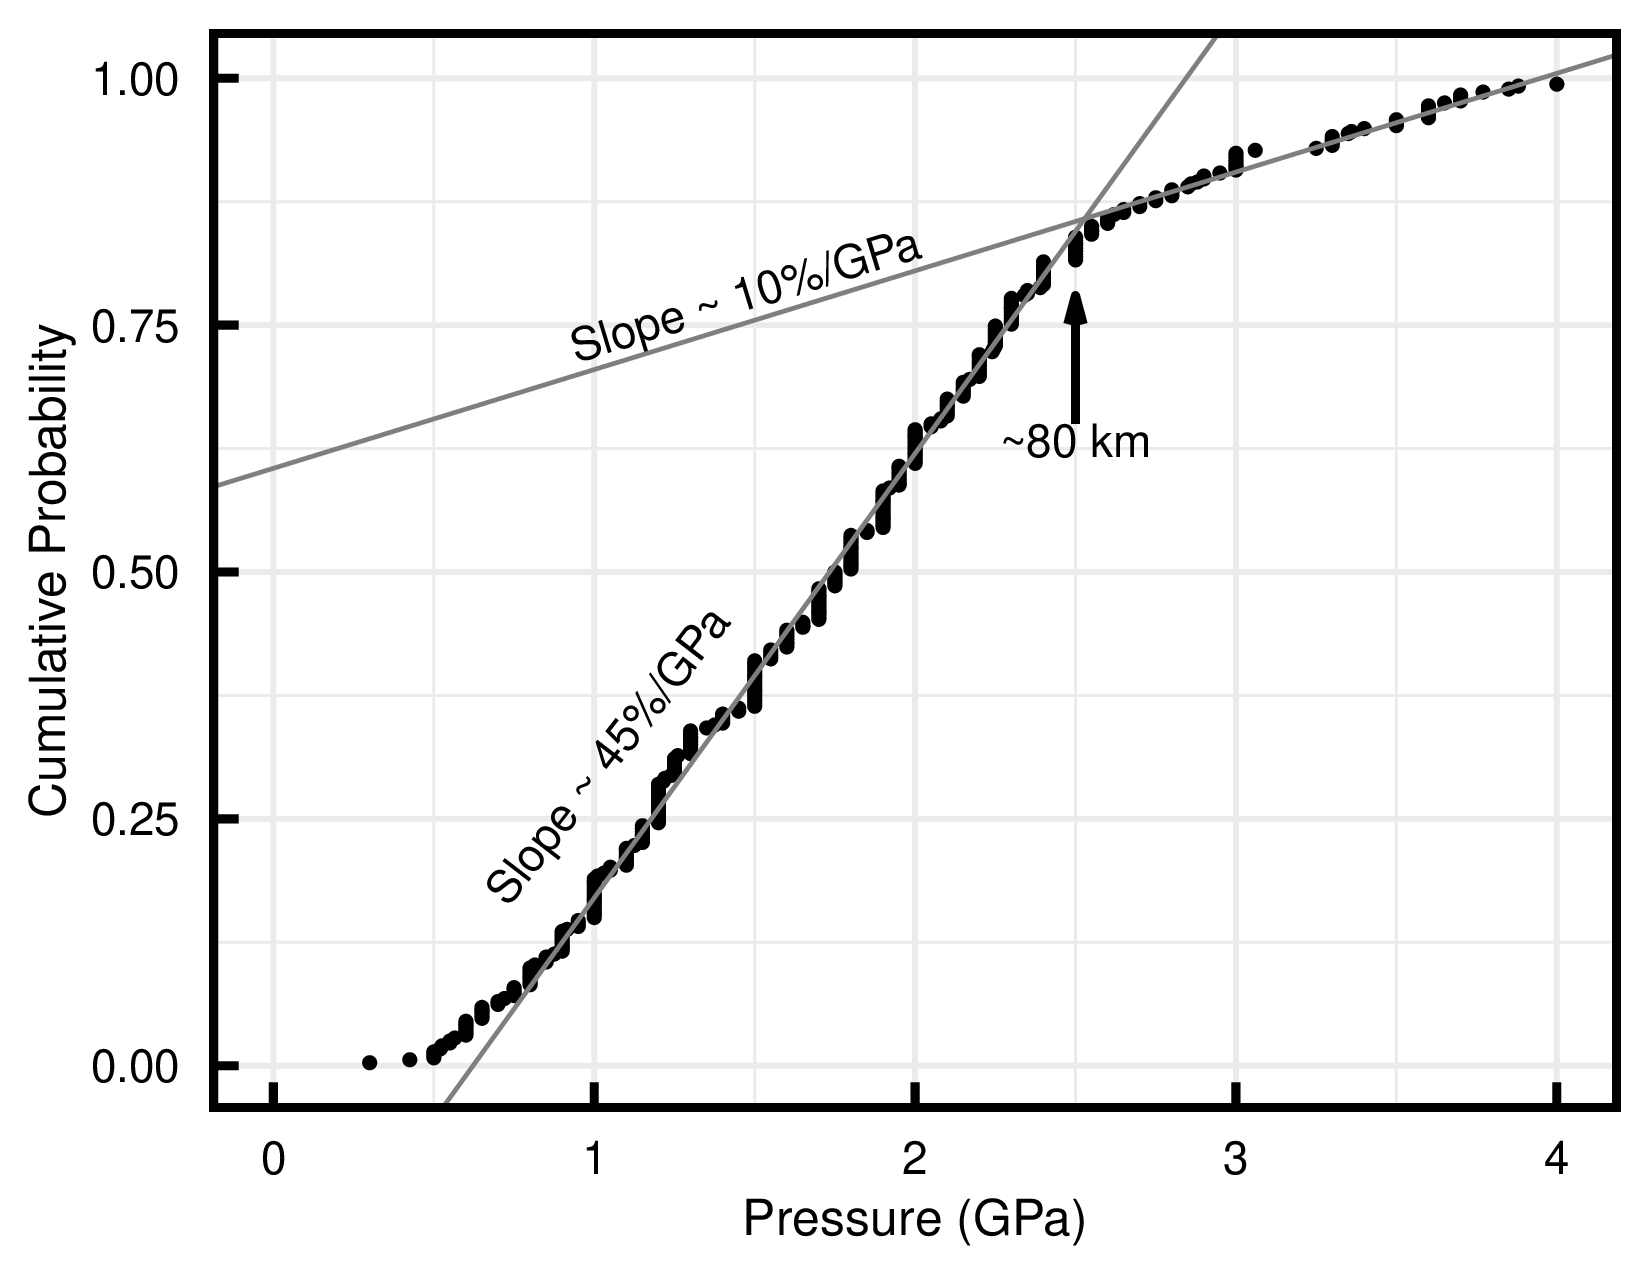
\includegraphics[width=0.5\textwidth,  trim={0 0 0 0}]{figs/FigS2.png}
 \caption{Cumulative probability versus peak metamorphic pressures for metamorphic rocks exhumed from subduction zones. The break in slope at ca. 2.5 $GPa$ (ca. 80 $km$) suggests that the relative probability that a rock will exhume from pressures less than ca. 2.5 $GPa$ is substantially greater (steeper slope) than for higher pressure rocks (shallower slope). Nearly all rocks exhumed from pressures greater than ca. 2.5 $GPa$ derive from continental crust and were exhumed during collision. Paucity of data below 0.5 $GPa$ reflects sampling bias because these rocks are at best incipiently metamorphosed and not conducive to thermobarometry. Data are from \protect\cite{Penniston2015}.}
 \label{FigureS2}
\end{figure}

\begin{figure}[H]
 \centering
 \includegraphics[width=\textwidth,  trim={0 0 0 0}]{figs/FigS3.png}
 \caption{Visualization of rock type (a), log viscosity (b), log shear heating (c), effective P\'{e}clet number (d), log stress (e), density (f), and log strain rate (g) for the standard model cdf78 at 1.64 $Ma$. Early subduction is facilitated by the prescribed initial weak layer (high pore fluid pressure) cutting the lithosphere. The P\'{e}clet number in the mantle wedge is less than the P\'{e}clet number of the slab. Heat sinks from the upper mantle wedge to lower in the mantle through thermal diffusion into the slab and advection of that heat downwards by the slab. Antigorite stabilizes to deeper depths.}
 \label{FigureS3}
\end{figure}

\begin{figure}[H]
 \centering
 \includegraphics[width=\textwidth,  trim={0 0 0 0}]{figs/FigS4.png}
 \caption{Visualization of rock type (a), log viscosity (b), log shear heating (c), effective P\'{e}clet number (d), log stress (e), density (f), and log strain rate (g) for the standard model cdf78 at 5.05 $Ma$. By 5 $Ma$ balanced is achieved between heat sinking from the upper mantle wedge to lower parts of the mantle by strong advection of heat in the circulating part of the mantle wedge. The ratio of mantle-slab P\'{e}clet number increases abruptly at approx. 80-90 $km$ depth from the surface. A feedback has already developed\textemdash heat advection destabilizing antigorite, resulting in slab-mantle coupling, driving mantle wedge circulation, advecting heat towards the coupling region quicker than can be sunk by the slab.}
 \label{FigureS4}
\end{figure}

\begin{figure}[H]
 \centering
 \includegraphics[width=\textwidth,  trim={0 0 0 0}]{figs/FigS5.png}
 \caption{Visualization of rock type (a), log viscosity (b), log shear heating (c), effective P\'{e}clet number (d), log stress (e), density (f), and log strain rate (g) for the standard model cdf78 at 9.93 $Ma$. The geodynamics and thermal structure remain approximately constant from 5 $Ma$ (cf. Fig~\ref{FigureS4}). The system remains in steady state for as long as enough water is supplied to the upper mantle wedge to stabilize antigorite.}
 \label{FigureS5}
\end{figure}

\newpage

\acknowledgments
We thank the Geophysical Fluid Dynamics group at the Institut für Geophysik, ETH Zürich, for their computing resources and invaluable instruction, discussion, and support on the numerical modelling methods. We also thank P. Agard, L. Le Pourhiet, and their students at ISTeP, Sorbonne Université, for suggestions on the numerical modelling methods and discussions that greatly enhanced this study. We thank two anonymous reviewers for their helpful comments and suggestions, which prompted our formulation of an effective P\'{e}clet number and improved the manuscript. This work was supported by the National Science Foundation grant OIA1545903 to M. Kohn, S. Penniston-Dorland, and M. Feineman. Datasets and tools for reproducing the research in this study are available at the official data repository (\url{https://doi.org/10.17605/OSF.IO/ZJAC3} ) or at \url{https://github.com/buchanankerswell/kerswell_et_al_coupling}.

\bibliography{assets/ref}


\end{document}
